\chapter{Translation Pipeline} \label{chap:pipeline}
In this chapter, I evaluate the ability of large language models (LLMs) to translate Linear B into Ancient Greek. 
The full pipeline proceeds as follows:

\begin{itemize}[leftmargin=2em]
  \item \textbf{Vocabulary extraction.} Gather every distinct word form attested in the Linear B documents (after cleaning/normalization).
  \item \textbf{Brute-force cognates.} For forms not already covered by our dataset, run the brute-force search against the Ancient Greek lexicon to obtain initial candidates (detailed in Section \ref{sec:bruteforce-cognates}).
  \item \textbf{Candidate aggregation.} For each word, collect possible cognates from: (i) the dataset's suggested cognates, (ii) the raw output of the cognate-matching model trained on our dataset, together with the output of all decoding modes, and (iii) a version of the cognate matcher retrained on the enlarged set. Duplicates are removed from the candidate set.
  \item \textbf{Auxiliary signals.} Train the Linear-SVM auxiliary classifiers on their labeled sets, then predict part of speech, noun type, and inflection for every word in the corpus.
  \item \textbf{Logograms.} Map logograms to their conventional readings/values and include these as fixed translations.
  \item \textbf{LLM prompting.} For each item, assemble a structured prompt containing: the Linear B form, the deduplicated cognate candidates, auxiliary predictions, and relevant morphological guidance. The LLM is asked to (a) select or propose the most plausible Ancient Greek reconstruction, and (b) provide an English translation.
  If the information provided with the prompt is sufficient, the LLM should be able to reconstruct the right inflection for each term and disambiguate the sentence.
\end{itemize}

\begin{figure}[H]
    \begin{adjustbox}{center}
        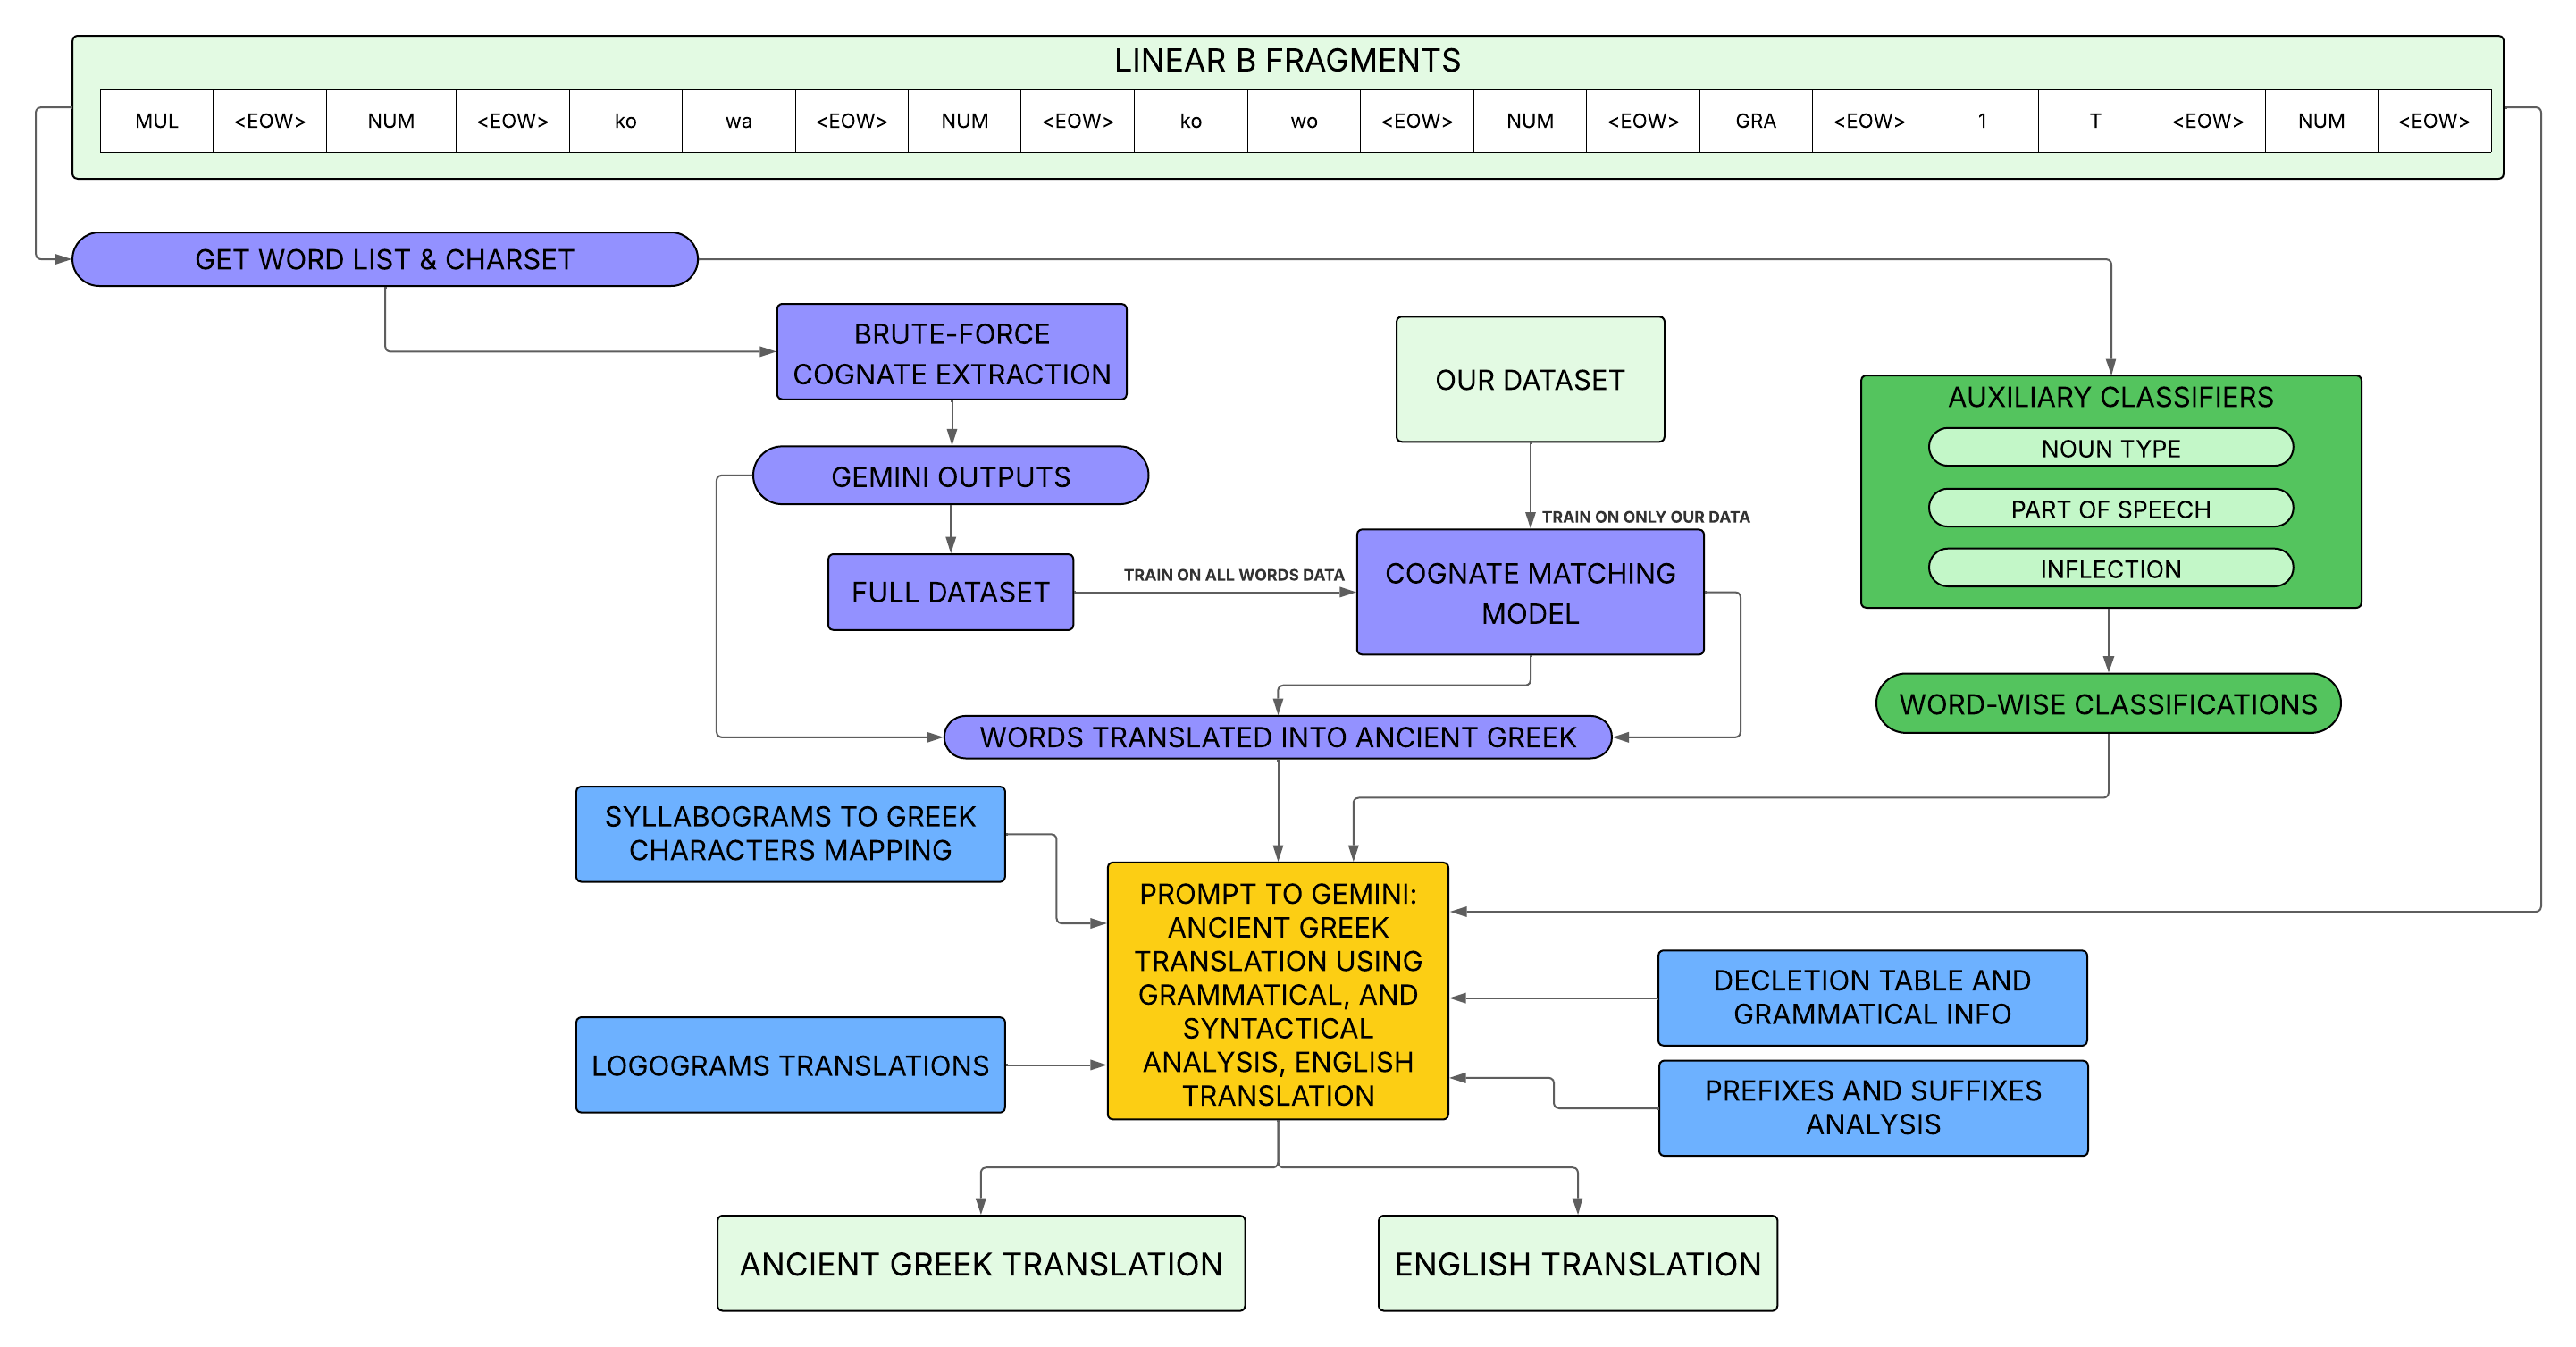
\includegraphics[width=1.2\textwidth]{Images/pipeline.png}
    \end{adjustbox}
    \caption{Overview of the translation pipeline from Linear B to Ancient Greek.}
    \label{fig:pipeline}
\end{figure}

\section{Prompt Design} \label{sec:final-prompt}
This time, instead of a single prompt, the information was given to the large language model using a series of structured messages, each with a specific role.

\paragraph{Historical Context.}
The first message provided to the model was a simple historical context on Linear B and Ancient Greek relationship.
It underlines the fact that Linear B is an early form of Greek, written with a syllabic script, and its administrative nature.
This message was fixed for all words.

\paragraph{Syllabogram Matching.}
The second message contained the Linear B syllabograms and their closest Ancient Greek equivalents, predicted by Luo's model.
It associates to each Linear B syllabogram a list of symbols that could represent it in its Ancient Greek correspondence.
For example, the Linear B syllabogram \textlinb{\Bpa} (pa) is associated with the Ancient Greek letters \textgreek{π}, \textgreek{φ}, and \textgreek{α}, as it usually corresponds to "\textgreek{πα}" or "\textgreek{φα}" syllables.
This was also fixed for all words.

\paragraph{Grammatical Information.}
The third message provided auxiliary grammatical information, such as Linear B declension tables, and additional information about adjectives and verbs, like in the prompt described in Section \ref{sec:aux-dataset}.

\paragraph{Task Definition.}
The fourth message formalized the task. The model receives the Linear~B document as a sequence of tokenized word forms; for each word it is given (i) the aggregated set of candidate Ancient Greek cognates, (ii) auxiliary predictions (part of speech, noun type when applicable, and inflection when applicable), and (iii) a completeness label.
The completeness label is derived from the share $p\!\in\![0,1]$ of occurrences marked as "complete" in the corpus and is bucketed at fixed cutoffs:
\emph{Always Complete} ($p=1$), \emph{Mostly Complete} ($p \geq \frac{2}{3}$), \emph{Uncertain} ($\frac{1}{3} < p < \frac{2}{3}$), \emph{Mostly Incomplete} ($0< p \leq \frac{1}{3}$), \emph{Incomplete} ($p=0$).

The prompt instructs the model on how to complete the translation task, the main steps being:
\begin{itemize}
  \item \textbf{Grammatical analysis.} The first step is to analyze the grammatical features of the Linear B document, separating the words into adjectives, nouns, verbs, and adverbs, and reconstructing the inflection of each noun and adjective, as well as the conjugation of each verb.
  \item \textbf{Syntactic analysis.} The second step is to analyze the document's structure by identifying its sentences and distinguishing the subjects, verbs, and objects mentioned in them.
  \item \textbf{Discourse analysis.} The third step is to analyze the discourse, examining subordinate clauses and establishing coherent logical connections.
  \item \textbf{Linguistic authenticity.} The fourth step is to ensure the selection of an Ancient Greek cognate that preserves morphological patterns and is plausible given the corresponding Mycenaean Greek form.
  \item \textbf{Semantic coherence.} The last step is to ensure that the translation is semantically coherent with the administrative nature of the Linear B documents.
\end{itemize}

These are common steps in translation and linguistic analysis, but they are particularly important in this context due to the similarity between Linear B inflected forms.
The LLM is finally asked given some quality assurance criteria, reflecting the needs of the task, and instructed to use the chain-of-thought technique to reason step by step and refine its translation.

\paragraph{Examples.}
The last information given to the model is a series of examples of translated Linear B fragments.
These examples are selected from a small set of documents provided by Chris Tselentis, together with his Linear B lexicon \cite{tselentis}.

These examples are very short, but they cover a variety of linguistic phenomena and be representative of the administrative purpose of the documents.
The following examples were used:

\begin{enumerate}
  \item \textbf{PY Eb 895+906}: This brief document contains a subordinate clause introduced by a participial form.
  Therefore, it provides key features of Linear B clause structure. \\
  \textbf{Linear B original}: \textlinb{\Ba\Bi\Bqe\Bu} \textlinb{\Be\Bke\Bqe} \textlinb{\Bke\Bke\Bme\Bna} \textlinb{\Bko\Bto\Bna} \textlinb{\Bko\Bto\Bno\Bko} \textlinb{\Bto\Bso\Bde} \textlinb{\Bpe\Bmo} \textlinb{\BPwheat} \textlinb{\BPvolcd} \textlinb{\BNvi}\\
  \textbf{Linear B text}: a-i-qe-u e-ke-qe ke-ke-me-na ko-to-na ko-to-no-o-ko to-so-de pe-mo GRA T 6 \\
  \textbf{Greek translation}: \textgreek{Αἰγεὺς κτοινόοχος ἔχει τε κεκειμένα κτοίνα τοσόνδε σπέρμον ΣΙΤΟΣ Τ 6} \\
  \textbf{English translation}: Aigeus, the plot owner, who owns a communal plot; so much grain: 6 'T' units of wheat. \\
  
  \begin{figure}[H]
    \centering
    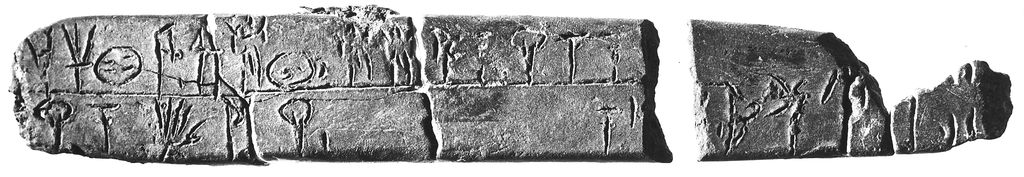
\includegraphics[width=0.7\textwidth]{Images/4901.png} % Adjust width and filename
    \caption{Picture of the original document PY Eb 895+906.}
    \label{fig:example1}
  \end{figure}

  \item \textbf{PY Ta 711}: This fragment is very short as well. It is excerpted from a longer document, whose translation will be fully evaluated in Section \ref{sec:translations}.
  However, it also contains a subordinate clause, introduced here by a particle.
  Moreover, it underscores the importance of grammatical and syntactic analysis, as the subject and the object of the sentence exhibit overlapping inflectional endings. \\
  \textbf{Linear B original}: \textlinb{\Bo\Bwi\Bde} \textlinb{\Bpu\Bke\Bqi\Bri} \textlinb{\Bo\Bte} \textlinb{\Bwa\Bna\Bka} \textlinb{\Bte\Bke} \textlinb{\Bau\Bke\Bwa} \textlinb{\Bda\Bmo\Bko\Bro}\\
  \textbf{Linear B text}: o-wi-de phu-ke-qi-ri o-te wa-na-ka te-ke au-ke-wa da-mo-ko-ro \\
  \textbf{Greek translation}: \textgreek{ὀ-εἶδε Φυγεκλής ὅτε ἄναξ θῆκε Αὐγέαν δάμοκλον} \\
  \textbf{English translation}: Phygekles witnessed when the king appointed Augeus as damoklos. \\

  \begin{figure}[H]
    \centering
    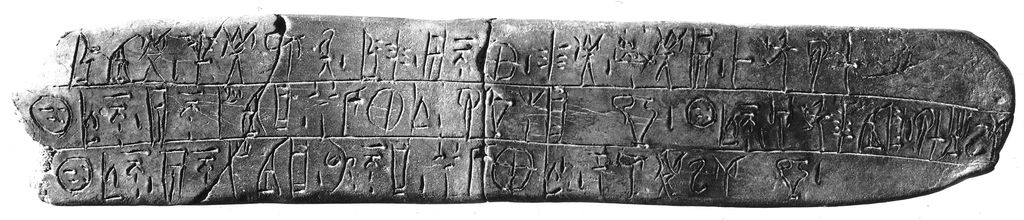
\includegraphics[width=0.8\textwidth]{Images/5350.png} % Adjust width and filename
    \caption{Picture of the original document PY Ta 711.}
    \label{fig:example2}
  \end{figure}

  \item \textbf{PY Ae 303}: This very brief document, like the previous two, illustrates long-distance agreement: the attributive adjective and the noun it modifies stand far apart in the line.
This word-order freedom is common in Ancient Greek and underscores why careful grammatical and logical analysis is essential. \\
  \textbf{Linear B original}: \textlinb{\Bi\Bje\Bro\Bjo} \textlinb{\Bpu\Bro} \textlinb{\Bi\Bje\Bre\Bja} \textlinb{\Bdo\Be\Bra} \textlinb{\Be\Bne\Bka} \textlinb{\Bku\Bru\Bso\Bjo} \textlinb{\BPwoman} \textlinb{\BNx\BNiv}\\
  \textbf{Linear B text}: i-je-ro-jo pu-ro i-je-re-ja do-e-ra e-ne-ka ku-ru-so-jo MUL 14 \\
  \textbf{Greek translation}: \textgreek{Πύλος: ιερείας δούλαι ένεκα χρυσοίο ιεροίο ΓΥΝΗ 14} \\
  \textbf{English translation}: Pylos: slaves of the priestess for the sake of sacred gold, 14 women. \\

  \begin{figure}[H]
    \centering
    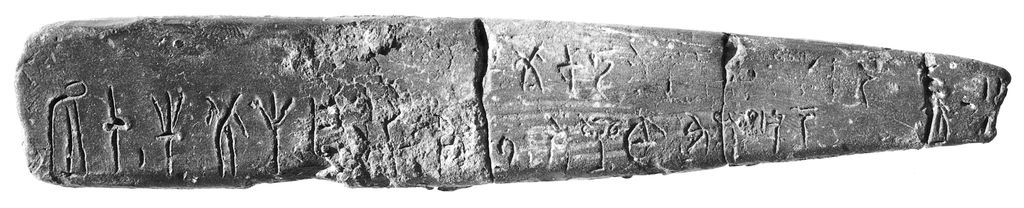
\includegraphics[width=0.7\textwidth]{Images/4684.png} % Adjust width and filename
    \caption{Picture of the original document PY Ae 303.}
    \label{fig:example3}
  \end{figure}

\end{enumerate}

\paragraph{Outputs}
The model is expected to output a JSON object with three fields:
\begin{itemize}
  \item \texttt{Ancient Greek}: the reconstructed Ancient Greek translation of the Linear B document.
  \item \texttt{English}: the English translation of the Linear B document.
  \item \texttt{Reasoning}: a detailed reasoning process, following the steps outlined in the task definition, explaining how the model arrived at its translations.
\end{itemize}

\section{Results} \label{sec:translations}
In this section, the outputs of the Translation Pipeline will be presented and compared with existing translations of the same documents, provided by Tselentis' lexicon \cite{tselentis}.

The parameters used for the LLM are the following: Gemini~2.5~Flash, with temperature 0.1, top-p 0.95, and top-k 0.4.

The evaluation will focus on the quality of the Ancient Greek reconstructions and the accuracy of the English translations.
Moreover, errors will be analyzed and the reasoning provided by the model will be assessed to understand the possible causes of mistakes.
A small sample of documents will not be assessed, as it was used as examples in the prompt (see Section \ref{sec:final-prompt}).

\subsection{Evaluated Documents}
The documents selected for evaluation are the following:
\begin{enumerate}[label=(\roman*)]
\item PY Ta 711
\item KN Ra 1540
\item PY Jn 310
\item PY Jn 829
\item KN So 4439
\item KN Sd 4404
\item PY An 657
\item PY TA 641
\item PY Er 312
\item KN Fp 1+31
\item PY Ab 573
\item PY Un 718
\end{enumerate}

The fragments of the documents whose translations were provided by Tselentis are highlighted in \emph{italics}.

\subsubsection{PY Ta 711}
This document was already presented as part of the examples in the prompt to the LLM.
However, only the first fragment was used as an example, while the rest of the document was reserved for evaluation. \\
\textbf{Linear B text}: \textit{o-wi-de phu-ke-qi-ri o-te wa-na-ka te-ke au-ke-wa da-mo-ko-ro} qe-ra-na wa-na-se-wi-ja qo-u-ka-ra ko-ki-re-ja *204VAS 1 qe-ra-na a-mo-te-wi-ja ko-ro-no-we-sa qe-ra-na wa-na-se-wi-ja ku-na-ja qo-u-ka-ra 1 to-qi-de-we-sa *204VAS 1 \\
\textbf{Greek translation}: \textgreek{ὀ-εἶδε Φυγεκλής ὅτε ἄναξ θῆκε Αὐγέαν δάμοκλον. κερανα ϝανασεϝια βουκαρα κοχλιρεια ΣΚΕΥΟΣ 1. κερανα αρμοθηϝια κορωνοϝέσσα. κερανα ϝανασεϝια γυναια βουκαρα 1. τροπιδϝέσσα ΣΚΕΥΟΣ 1.} \\
\textbf{English translation}: Phygekles witnessed when the king appointed Augeus as damoklos. A royal, ox-head-shaped, spiral-decorated krater (vessel): 1. A krater with fittings, with a handle. A royal, female, ox-head-shaped krater: 1. A spiral-designed vessel: 1.

\paragraph{Analysis.}
After the first narrative clause, the document lists four types of vessels.
The LLM correctly reconstructs the context and provides a meaningful and coherent translation.

Allow me to analyze the four vessel descriptions in detail:
\begin{itemize}
\item The word \textlinb{\Bqe\Bra\Bna} (qe-ra-na) is correctly identified as a noun, and the LLM selects the Ancient Greek cognate \textgreek{κερανα}.
However, the expected form would definitely be \textgreek{κέρνα}, the nominative/accusative plural of \textgreek{κέρνος}, which is used in Ancient Greek to denote a sacred vessel.
\item The word \textlinb{\Bwa\Bna\Bse\Bwi\Bja} (wa-na-se-wi-ja) is correctly identified as an adjective, and the LLM selects an Ancient Greek form that closely echoes the original Linear B word: \textgreek{ϝανασεϝια}, rather than the Ancient Greek \textgreek{αναξια}.
Other adjectives referring to this vessel are \textlinb{\Bqo\Bu\Bka\Bra} (qo-u-ka-ra, "ox-head shaped") and \textlinb{\Bko\Bi\Bre\Bja} (ko-ki-re-ja, "spiral-decorated").
The first is associated with a synthetic compound Ancient Greek form composed of \textgreek{βους} "ox" and \textgreek{καρα} "head", while the second is translated as \textgreek{κοχλιρεια}, an adjective derived from \textgreek{κοχλος}, "spiral-shaped shell", sharing the root with Ancient Greek \textgreek{κοχλιοειδης/κοκλιωδης}.
\item The following vessel is associated with the adjectives \textlinb{\Bko\Bro\Bno\Bwe\Bsa} (ko-ro-no-we-sa), meaning the krater is provided with handles (from Ancient Greek \textgreek{κορωνη}), and \textlinb{\Ba\Bmo\Bte\Bwi\Bja} (a-mo-te-wi-ja), linked to the concept of "fittings" or chariot-related terms (from Ancient Greek \textgreek{αρμος} "joint" and \textgreek{αρμα} "chariot"), even though no fully satisfactory Greek correspondence can be found.
\item The third vessel is again described as royal and ox-head shaped, but the third adjective is \textlinb{\Bku\Bna\Bja} (ku-na-ja), from Ancient Greek \textgreek{γυναια}, "womanly".
\item The last vessel is described as \textlinb{\Bto\Bqi\Bde\Bwe\Bsa} (to-qi-de-we-sa), "spiral-designed", from Ancient Greek \textgreek{τροπιδϝέσσα}, derived from \textgreek{τροπις}, which actually means "keel", and whose connection to spirals is only indirect through the notion of turning or curving, but is also confirmed by Tselentis' lexicon \cite{tselentis}.
\end{itemize}
Overall, the LLM's English translation is quite accurate, while the Ancient Greek reconstruction still retains Linear B features.

Here I report an improved version of the Greek translation, highlighting in red the adjustments. For the English translation, no changes are needed. \\
\textbf{Greek translation}: \textcolor{red}{\textgreek{οἶδε}} \textgreek{Φυγεκλής ὅτε ἄναξ θῆκε Αὐγέαν δάμοκλον.} \textcolor{red}{\textgreek{κέρνα ἀναξία}} \textgreek{βουκάρα} \textcolor{red}{\textgreek{κοχλιοειδή}} \textgreek{ΣΚΕΥΟΣ 1.} \textcolor{red}{\textgreek{κέρνα}} \textgreek{αρμοθήϝια κορωνοϝέσσα}. \textcolor{red}{\textgreek{κέρνα ἀναξία}} \textgreek{γυναίκα βουκάρα 1. τροπιδϝέσσα ΣΚΕΥΟΣ 1.}

The picture of this document is shown in Figure \ref{fig:example2}.

\subsubsection{KN Ra 1540}
This document is a very short inventory entry of a single item: swords. \\
\textbf{Linear B text}: \textit{to-sa pa-ka-na PUG 50} \\
\textbf{Greek translation}: \textgreek{τόσα φάσγανα ΦΑΣΓΑΝΑ 50.} \\
\textbf{English translation}: So many swords: 50 SWORDS.
\paragraph{Analysis.}
In this case, the LLM correctly reconstructs the whole document, due to its simplicity.
The words \textlinb{\Bto\Bsa} (to-sa) and \textlinb{\Bpa\Bka\Bna} (pa-ka-na) are correctly identified as a quantifier and a noun, respectively.
They are translated into their corresponding Ancient Greek cognates: \textgreek{τόσα} and \textgreek{ϝάσγανα}, the accusative plural of \textgreek{ϝάσγανον}, "sword".
The English translation is also accurate, therefore no changes are needed.

\begin{figure}[H]
  \centering
  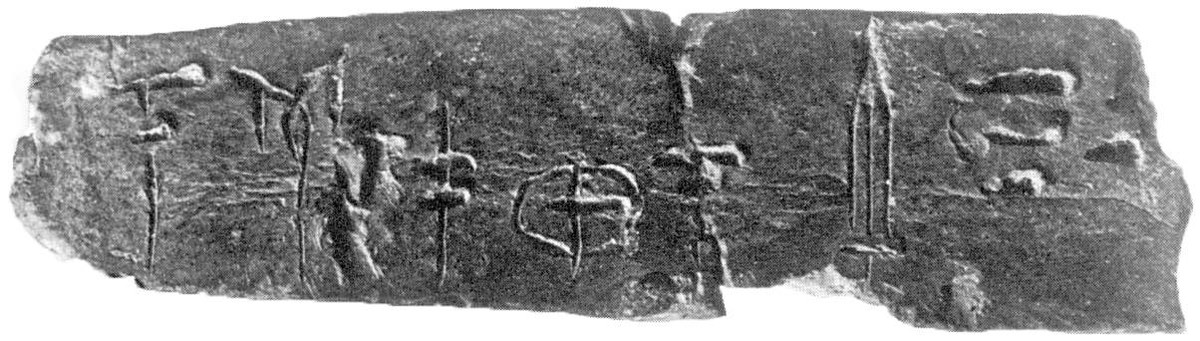
\includegraphics[width=0.7\textwidth]{Images/250.png} % Adjust width and filename
  \caption{Picture of the original document KN Ra 1540.}
  \label{fig:doc2}
\end{figure}

\subsubsection{PY Jn 310} \label{doc:pyjn310}
Tselentis provides a translation for only a fragment of this document, which is quite long.
However, the LLM appears able to handle the entire text well, thanks to its repetitive structure. \\
\textbf{Linear B text}: a-ke-re-wa [...] ka-ke-we ta-ra-si-ja e-ko-te ti-qa-jo AES M 1 N 2 qe-ta-wo AES M 1 N 2 ai-so-ni-jo AES M 1 N 2 ta-mi-je-u AES M 1 N 2 e-u-ru-wo-ta AES M 1 N 2 e-u-do-no AES M 1 N 2 po-ro-u-te-u AES M 1 N 2 wi-du-wa-ko AES M 1 N 2 to-so-de a-ta-ra-si-jo ka-ke-we [...] pa-qo-si-jo 1 ke-we-to 1 [...] 1 [...] pe-ta-ro 1 to-so-de do-e-ro ke-we-to-jo 1 i-wa-ka-o 1 pa-qo-si-jo-jo 1 po-ro-u-te-wo 1 a [...] \textit{po-ti-ni-ja-we-jo ka-ke-we ta-ra-si-ja e-ko-te} i-ma-di-jo [...] AES M 3 tu-ke-ne-u AES M 3 AES M 3 i-wa-ka AES M 3 a-ta-ra-si-jo phu-si-ja-ko 1 \\
\textbf{Greek translation}: \textgreek{Ἀγρεϝα [...] χαλκεϝες ταλανσία ἔχοντες: Τιθαιος ΧΑΛΚΟΣ M 1 N 2, Κεταϝος ΧΑΛΚΟΣ M 1 N 2, Αἰσώνιος ΧΑΛΚΟΣ M 1 N 2, Ταμιεύς ΧΑΛΚΟΣ M 1 N 2, Εὐρυϝότας ΧΑΛΚΟΣ M 1 N 2, Εὔδονος ΧΑΛΚΟΣ M 1 N 2, Πλουτεύς ΧΑΛΚΟΣ M 1 N 2, Ϝιδυϝακος ΧΑΛΚΟΣ M 1 N 2. Τόσοςδε ἀταλανσίοι χαλκεϝες [...]: Παμφίσιος 1, Κηϝετος 1, [...] 1, [...] 1, Πέταλος 1. Τόσοςδε δοῦλοι: Κηϝετοιο 1, Ἰϝακαο 1, Παμφισίοιο 1, Πλουτέϝος 1. Ἀ [...] Ποτνιάϝειοι χαλκεϝες ταλανσία ἔχοντες: Ἱμαδιος [...] ΧΑΛΚΟΣ M 3, Τυχενεύς ΧΑΛΚΟΣ M 3, ΧΑΛΚΟΣ M 3, Ἰϝακα ΧΑΛΚΟΣ M 3. Ἀταλανσίοι: Φυσίαρχος 1.} \\
\textbf{English translation}: Agrewa: [...] bronze-smiths having allotment: Tithaios: BRONZE M 1 N 2, Ketawo: BRONZE M 1 N 2, Aisonios: BRONZE M 1 N 2, Tamieus: BRONZE M 1 N 2, Eurywotas: BRONZE M 1 N 2, Eudonos: BRONZE M 1 N 2, Plouteus: BRONZE M 1 N 2, Widuwako: BRONZE M 1 N 2. Total bronze-smiths without allotment [...]: Pamphisios 1, Kewetos 1, [...] 1, [...] 1, Petalos 1. Total slaves: Of Kewetos 1, Of Iwaka 1, Of Pamphisios 1, Of Plouteus 1. A [...] Potnia-related bronze-smiths having allotment: Himadios [...] BRONZE M 3, Tucheneus: BRONZE M 3, BRONZE M 3, Iwaka: BRONZE M 3. Without allotment: Physiarchos 1.

\paragraph{Analysis.}
This document is an administrative record from the site of Pylos, listing bronze-smiths, their allotments of bronze, and associated personnel (slaves).
It is structured into several sections based on the status and affiliation of the craftsmen.
Most words occurring in the document are proper nouns, for which the Ancient Greek correspondence is a simple transliteration.
The most notable common words are:
\begin{itemize}
\item \textlinb{\Bka\Bke\Bwe} (ka-ke-we), "bronze-smith", from Ancient Greek \textgreek{χαλκεύς}, correctly identified as a noun by the LLM and transliterated in a form preserving the digamma (\textgreek{χαλκεϝες} rather than \textgreek{χαλκεῖς}).
\item \textlinb{\Bta\Bra\Bsi\Bja} (ta-ra-si-ja), "allotment", from Ancient Greek \textgreek{ταλανσία}, also correctly identified as a noun.
It shares its root with \textgreek{τάλαντον}, "talent", a unit of weight (and later currency), with the sense of "allotment" deriving from a weight of metal assigned to a worker.
\item \textlinb{\Be\Bko\Bte} (e-ko-te), "having", from Ancient Greek \textgreek{ἔχοντες}, the nominative plural masculine present active participle of \textgreek{ἔχω}, "to have".
Another straightforward form is \textlinb{\Bdo\Be\Bro} (do-e-ro), from Ancient Greek \textgreek{δοῦλοι}, the nominative plural masculine of \textgreek{δοῦλος}, "slave".
\item Both \textlinb{\Bto\Bso\Bde} (to-so-de) and \textlinb{\Ba\Bta\Bra\Bsi\Bjo} (a-ta-ra-si-jo) are interpreted as nominative plural adjectives referring to the bronze-smiths.
The former means "so many" or "total", from Ancient Greek \textgreek{τοσόσδε}, while the latter means "without allotment", from Ancient Greek \textgreek{ἀταλανσίος}, built from the negative prefix \textgreek{ἀ-} and \textgreek{ταλανσία}, "allotment".
\item The translation of \textlinb{\Bpo\Bti\Bni\Bja\Bwe\Bjo} (po-ti-ni-ja-we-jo) is problematic in this context.
While the LLM interprets it as a nominative plural associated with the bronze-smiths, Tselentis gives it a locative neuter value, linking it to the initial word \textlinb{\Ba\Bke\Bre\Bwa} (a-ke-re-wa), a toponym.
Accordingly, while the LLM's rendering remains vague, Tselentis' proposal is to read it as "at the place of Potnia", associating it with \textgreek{ποτνιάδειον}.
\end{itemize}

The LLM's English translation is quite accurate, although it reflects the issue with the word "po-ti-ni-ja-we-jo".
For both translations, I report an improved version below, highlighting in red the adjustments and in blue the actual mistakes. \\
\textbf{Greek translation}: \textgreek{Ἀγρεϝα [...]} \textcolor{red}{\textgreek{χαλκεῖς}} \textgreek{ταλανσία ἔχοντες: Τιθαιος ΧΑΛΚΟΣ M 1 N 2, Κεταϝος ΧΑΛΚΟΣ M 1 N 2, Αἰσώνιος ΧΑΛΚΟΣ M 1 N 2, Ταμιεύς ΧΑΛΚΟΣ M 1 N 2, Εὐρυϝότας ΧΑΛΚΟΣ M 1 N 2, Εὔδονος ΧΑΛΚΟΣ M 1 N 2, Πλουτεύς ΧΑΛΚΟΣ M 1 N 2, Ϝιδυϝακος ΧΑΛΚΟΣ M 1 N 2.} \textcolor{red}{\textgreek{Τοσοίδε}} \textgreek{ἀταλανσίοι} \textcolor{red}{\textgreek{χαλκεῖς}} \textgreek{[...]: Παμφίσιος 1, Κηϝετος 1, [...] 1, [...] 1, Πέταλος 1.} \textcolor{red}{\textgreek{Τοσοίδε}} \textgreek{δοῦλοι: Κηϝετοιο 1,} \textcolor{red}{\textgreek{Ἰϝακου}} \textgreek{1, Παμφισίοιο 1, Πλουτέϝος 1. Ἀ [...]} \textcolor{blue}{\textgreek{ποτνιάδειον}} \textcolor{red}{\textgreek{χαλκεῖς}} \textgreek{ταλανσία ἔχοντες: Ἱμαδιος [...] ΧΑΛΚΟΣ M 3, Τυχενεύς ΧΑΛΚΟΣ M 3, ΧΑΛΚΟΣ M 3,} \textcolor{red}{\textgreek{Ἰϝακας}} \textgreek{ΧΑΛΚΟΣ M 3. Ἀταλανσίοι: Φυσίαρχος 1.} \\
\textbf{English translation}: Agrewa: [...] bronze-smiths having allotment: Tithaios: BRONZE M 1 N 2, Ketawo: BRONZE M 1 N 2, Aisonios: BRONZE M 1 N 2, Tamieus: BRONZE M 1 N 2, Eurywotas: BRONZE M 1 N 2, Eudonos: BRONZE M 1 N 2, Plouteus: BRONZE M 1 N 2, Widuwako: BRONZE M 1 N 2. Total bronze-smiths without allotment [...]: Pamphisios 1, Kewetos 1, [...] 1, [...] 1, Petalos 1. Total slaves: Of Kewetos 1, Of \textcolor{red}{Iwakas} 1, Of Pamphisios 1, Of Plouteus 1. A [...] \textcolor{blue}{At the place of Potnia}: bronze-smiths having allotment: Himadios [...] BRONZE M 3, Tucheneus: BRONZE M 3, BRONZE M 3, \textcolor{red}{Iwakas}: BRONZE M 3. Without allotment: Physiarchos 1.

\begin{figure}[H]
  \centering
  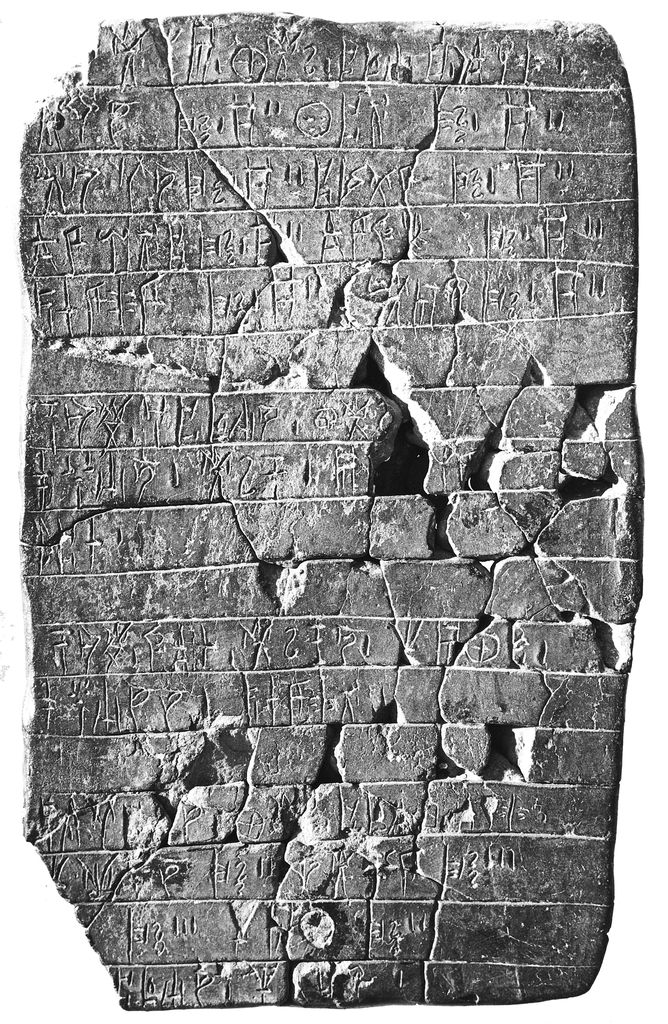
\includegraphics[width=0.55\textwidth]{Images/5057.png} % Adjust width and filename
  \caption{Picture of the original document PY Jn 310.}
  \label{fig:doc3}
\end{figure}

\subsubsection{PY Jn 829}
This document records the quantities of bronze collected for a temple and for the production of arrows.
The opening clause names the givers and states the purpose of the collection.
The remainder lists the amounts of bronze associated with various mayors and deputy mayors.
Because the closing portion is long and highly repetitive, I excluded it from the analysis.
Tselentis' translation covers only part of the opening sentence. \\
\textbf{Linear B text}: jo-do-so-si ko-re-te-re du-ma-te-qe po-ro-ko-re-te-re-qe ka-ra-wi-po-ro-qe o-pi-su-ko-qe o-pi-ka-pe-e-we-qe \textit{ka-ko na-wi-jo pa-ta-jo-i-qe e-ke-si-qe ai-ka-sa-ma} pi-*82 ko-re-te AES M 2 po-ro-ko-re-te AES N 3 me-ta-pa ko-re-te AES M 2 po-ro-ko-re-te AES N 3 [...] \\
\textbf{Greek translation}: \textgreek{Ὡς δώσουσι κορητῆρες δῠμᾶτές τε προκορητῆρές τε κλαϝιφόροί τε ὀπίσυκοί τε ὀπικαπεῆϝές τε χαλκόν ναϝίον, παλταίοις τε ἔχεσσι τε αἰχμάς. Πίσαϝι: κορητήρ ΧΑΛΚΟΣ M 2, προκορητήρ ΧΑΛΚΟΣ N 3. Μετάπα: κορητήρ ΧΑΛΚΟΣ M 2, προκορητήρ ΧΑΛΚΟΣ N 3.} \\
\textbf{English translation}: Thus will give the mayors and magistrates and deputy mayors and key-bearers and overseers of figs and overseers of digging, temple bronze, and spearheads for the javelin-men and for the spears. Pisa: mayor, bronze M 2, deputy mayor, bronze N 3. Metapa: mayor, bronze M 2, deputy mayor, bronze N 3. 

\paragraph{Analysis.}
The first part of the document lists the officials responsible for collecting bronze for a temple and for the production of arrows.
The LLM correctly identifies the main terms in this section, but it struggles with a few specific titles.
In the second part, the LLM correctly recognizes the place names and the officials; however, it is uncertain whether these officials are the collectors or the recipients of the bronze.
Given the usual structure of Linear B documents, they are more likely the collectors, since the introductory clause states that the bronze will be given by the officials.

The main terms in the first part of the document are:
\begin{itemize}
  \item \textlinb{\Bjo\Bdo\Bso\Bi\Bsi} (jo-do-so-si), "thus will give", from Ancient Greek \textgreek{ὡς δώσουσι}, the 3rd person plural future active indicative of \textgreek{δίδωμι} "to give".
  \item A series of Mycenaean official titles, correctly treated as nouns by the LLM. The most frequent here are \textlinb{\Bko\Be\Bre\Bte\Bre} (ko-re-te-re) "mayors" and \textlinb{\Bpo\Bro\Bko\Be\Bre\Bte\Bre} (po-ro-ko-re-te-re) "deputy mayors".
  Although the latter is transparently the former with a \textgreek{προ-} prefix, I find no fully satisfactory classical Greek equivalent beyond a transliteration.
  \item Additional titles include \textlinb{\Bdu\Bma\Bte} (du-ma-te) "magistrates/dāmos officials", linked by Tselentis to \textgreek{δῆμος} "people"; \textlinb{\Bka\Bra\Bwi\Bpo\Bro} (ka-ra-wi-po-ro) "key-bearers", from \textgreek{κλείς} "key" and \textgreek{φέρω} "carry/bear"; \textlinb{\Bo\Bpi\Bsu\Bko} (o-pi-su-ko) "overseers of figs", from \textgreek{ἐπί} "over" and \textgreek{σῦκον} "fig"; and \textlinb{\Bo\Bpi\Bka\Bpe\Be\Bwe} (o-pi-ka-pe-e-we) "overseers of digging", from \textgreek{σκάπτω} "to dig".
  \item The first object of the collection is bronze destined for a temple: \textlinb{\Bka\Bko} (ka-ko) "bronze", from \textgreek{χαλκόν}, and its adjective \textlinb{\Bna\Bwi\Bjo} (na-wi-jo) "temple-/sacral-", from \textgreek{ναίος} "of a temple".
  \item The second object consists of spearheads for javelins and for spears.
  These are expressed by \textlinb{\Baiii\Bka\Bsa\Bma} (ai-ka-sa-ma) "spearheads", from \textgreek{αἰχμή} (used here in the plural accusative), and by \textlinb{\Bpa\Bta\Bjo\Bi} (pa-ta-jo-i) "for javelins", from \textgreek{παλτόν}, and \textlinb{\Be\Bke\Bsi} (e-ke-si) "for the spears", from \textgreek{ἔγχος} (dative plural).
  The LLM, however, misinterpreted \textit{pa-ta-jo-i}, treating it as an adjective ("javelin-using") rather than as the noun "javelins," likely due to a misclassification.  \item The first toponym \textlinb{\Bpi\Bswa} (pi-*82) contains an uncertain syllabogram whose phonetic value is commonly taken to be "swa".
  \item The remainder of the tablet simply enumerates toponyms together with the quantities of bronze associated with each \textit{ko-re-te} (mayor) and \textit{po-ro-ko-re-te} (deputy mayor).
\end{itemize}

Here I report an improved version of the translations, highlighting in red the adjustments. \\
\textbf{Greek translation}: \textgreek{Ὡς δώσουσι κορητῆρες δῠμᾶτές τε προκορητῆρές τε κλαϝιφόροί τε} \textcolor{red}{\textgreek{ἐπισυκοί}} \textgreek{τε} \textcolor{red}{\textgreek{ἐπισκαπηϝές}} \textgreek{τε χαλκόν ναϝίον,} \textcolor{blue}{\textgreek{παλτοῖς}} \textgreek{τε} \textcolor{red}{\textgreek{ἔγχεσι}} \textgreek{τε αἰχμάς.} \textcolor{red}{\textgreek{Πίσϝα:}} \textgreek{κορητήρ ΧΑΛΚΟΣ M 2, προκορητήρ ΧΑΛΚΟΣ N 3. Μετάπα: κορητήρ ΧΑΛΚΟΣ M 2, προκορητήρ ΧΑΛΚΟΣ N 3.} \\
\textbf{English translation}: Thus will give the mayors and magistrates and deputy mayors and key-bearers and overseers of figs and overseers of digging, bronze \textcolor{red}{for the temple}, and spearheads for the \textcolor{blue}{javelins} and for the spears. \textcolor{red}{Piswa}: mayor, bronze M 2, deputy mayor, bronze N 3. Metapa: mayor, bronze M 2, deputy mayor, bronze N 3.

\begin{figure}[H]
  \centering
  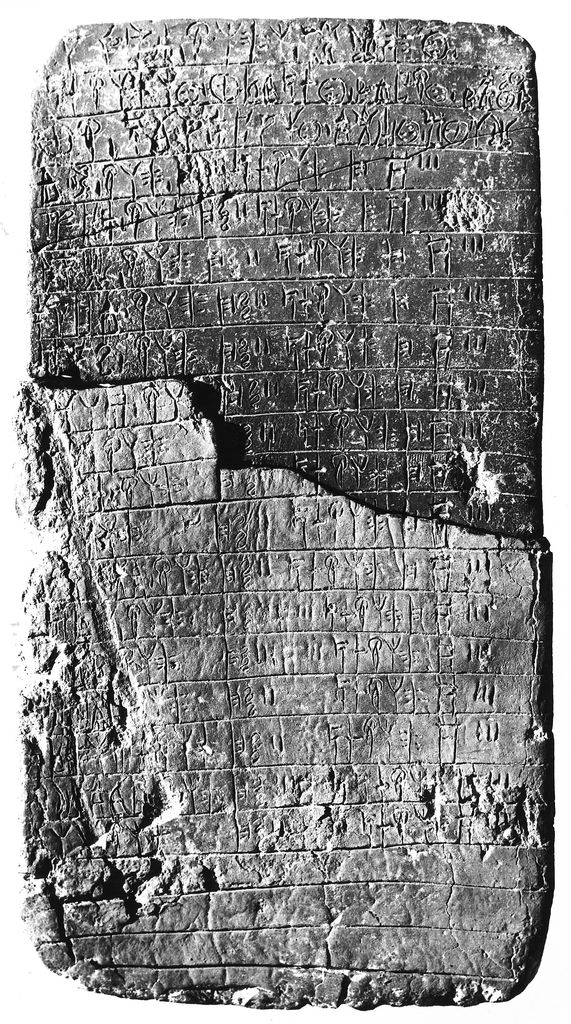
\includegraphics[width=0.35\textwidth]{Images/5072.png} % Adjust width and filename
  \caption{Picture of the original document PY Jn 829.}
  \label{fig:doc4}
\end{figure}

\subsubsection{KN So 4439} \label{doc:knso4439}
This very short document is an inventory of wheels.
Despite its brevity, it is actually one of the most challenging documents due to the presence of misleading words.
Tselentis provides the translation for the entire document. \\
\textbf{Linear B text}: \textit{a-mo-ta e-ri-ka te-mi-dwe-ta ROTA ZE 3 MO ROTA 1} \\
\textbf{Greek translation}: \textgreek{ἁρμότα ἑλίκαι τερμιδϝέντα: τροχοί ζεύγη 3, μόνος τροχός 1.} \\
\textbf{English translation}: Chariot fittings, willow (wood), rimmed: 3 pairs of wheels, 1 single wheel.

\paragraph{Analysis.}
The analysis of this document is particularly important, as it highlights the challenges posed by certain words that can easily mislead the LLM.
The main terms in this document are:
\begin{itemize}
  \item \textlinb{\Ba\Bmo\Bta} (a-mo-ta), "wheels/chariot", from Ancient Greek \textgreek{ἅρμα}, is the nominative plural and subject of the sentence.
  Despite its original meaning as "wheel", in classical Ancient Greek it came to denote the entire chariot.
  \item \textlinb{\Be\Bri\Bka} (e-ri-ka), "willow tree", from Ancient Greek \textgreek{ἑλικτός}, is here used as an adjective to describe the material of the wheels.
  However, the LLM misinterprets it as a noun, translating it as "willow". Moreover, its connection to the concept of "willow" is attested in Linear B, while in classical Ancient Greek \textgreek{ἑλικτός} means "twisted" or "curved".
  \item \textlinb{\Bte\Bmi\Bdwe\Bta} (te-mi-dwe-ta), "rimmed", from Ancient Greek \textgreek{τερμιόεις}, is correctly identified as an adjective by the LLM.
\end{itemize}
The LLM's English translation fails to capture the full meaning of the document, as it misunderstands the subject of the sentence and misinterprets the adjective referring to the material of the wheels.
Here I report an improved version of the translations, highlighting in red the adjustments and in blue the actual mistakes. \\
\textbf{Greek translation}: \textcolor{red}{\textgreek{ἅρματα}} \textcolor{blue}{\textgreek{ἑλικά}} \textcolor{red}{\textgreek{τερμιοέντα}}\textgreek{: τροχοί ζεύγη 3, μόνος τροχός 1.} \\ 
\textbf{English translation}: \textcolor{blue}{Wheels made of willow tree}, rimmed: 3 pairs of wheels, 1 single wheel.

\begin{figure}[H]
  \centering
  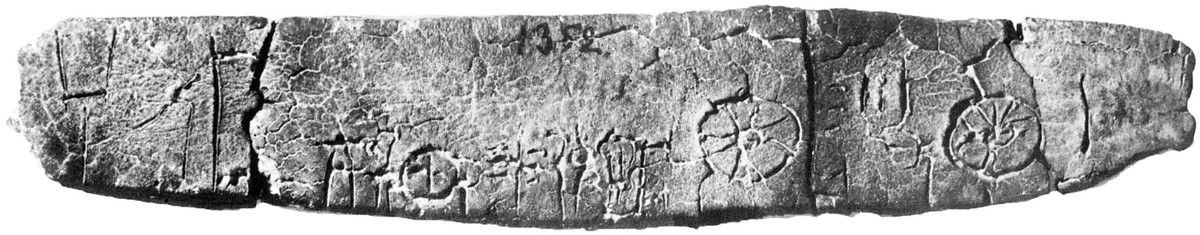
\includegraphics[width=0.7\textwidth]{Images/568.png} % Adjust width and filename
  \caption{Picture of the original document KN So 4439.}
  \label{fig:doc5}
\end{figure}

\subsubsection{KN Sd 4404}
This document is another inventory, this time for chariots.
Due to its fragmentary state, reconstructing its content is challenging.
Tselentis provides a translation for only the last fragment of the document. \\
\textbf{Linear B text}: jo [...] i-qo-e-qe wi-ri-ni-jo o-po-qo ke-ra-ja-pi o-pi-i-ja-pi CUR [...] \textit{i-qi-ja [...] ku-do-ni-ja mi-to-we-sa-e a-ra-ro-mo-te-me-na} po-ni-ki-ja BIG 1 \\
\textbf{Greek translation}: \textgreek{[...], ἱππο-ε-κες τε ϝίρινιοι ὀπωπω κεραίαφι ὀπίαιφι ΔΙΦΡΟΣ. [...] ἱππία Κυδωνία μιλτόϝεσσα ἀραρμοτhεμένη φοινικία ΔΙΦΡΟΣ 1.} \\
\textbf{English translation}: [...], and horse-equipped (parts), leathern eye-guards, with horn-like parts, with reins, a chariot. [...] A Cydonian, red-painted, fitted, red-dyed chariot: 1 chariot.

\paragraph{Analysis.}
Overall, the LLM performs well in recognizing the main words in the document, despite its fragmentary condition.
The main terms in this document are:
\begin{itemize}
  \item \textlinb{\Bi\Bqo\Be\Bqe} (i-qo-e-qe), which is linked to \textgreek{ἵππος} "horse". 
  It presents a strange \textit{-e} ending, and is interpreted as "horse-equipped parts", despite the fact that \textit{-qe} is usually a conjunction meaning "and".
  The peculiar ending might be dual ending, but this is only my speculation.
  \item \textlinb{\Bwi\Bri\Bni\Bo} (wi-ri-ni-jo) derives from \textgreek{ῥινός}, "leather", and it is an adjective associated with \textlinb{\Bo\Bpo\Bqo} (o-po-qo), "eye-guards", from \textgreek{ἐπί} and the root \textgreek{ὀπ-}, linked to sight, as in \textgreek{ὄψις}, "sight".
  \item \textgreek{κεραίαφι} (ke-ra-ja-pi) and \textgreek{ὀπίαιφι} (o-pi-i-ja-pi) are both in the instrumental terms, as indicated by the suffix \textit{-pi}, and mean "with horn-like parts" and "with reins".
  The former comes from Ancient Greek \textgreek{κέρας} "horn", while the latter has an uncertain etymology, possibly linked to \textgreek{ἡνία} "reins", combined with the \textgreek{ἐπί} prefix.
  \item \textlinb{\Bi\Bqi\Ba} (i-qi-ja) is the word for "chariot", from Ancient Greek \textgreek{ἵππια}, adjective related to \textgreek{ἵππος}, "horse".
  \item Three adjectives describe the chariot: \textlinb{\Bku\Bdo\Bni\Ba} (ku-do-ni-ja) is the toponym "Cydonia", from the ancient city of Cydonia in Crete.
  \textlinb{\Bmi\Bto\Bwe\Bsa\Be} (mi-to-we-sa-e) and \textlinb{\Bpo\Bni\Bki\Bja} (po-ni-ki-ja) mean "purple red-painted", from Ancient Greek \textgreek{μιλτός}, "red ochre" and \textgreek{φοινίκιος}, "phoenician", respectively. 
  \textlinb{\Ba\Bra\Bro\Bmo\Bte\Bme\Bna} (a-ra-ro-mo-te-me-na) is the passive participle of \textgreek{ἀρμόζω}, and means "fitted/assembled".
\end{itemize}
I provide an improved version of the translations below, highlighting in red the adjustments. \\
\textbf{Greek translation}: \textgreek{[...],} \textcolor{red}{\textgreek{ἱππω τε ϝρινιοι}} \textgreek{ὀπωπω κεραίαφι ὀπίαιφι ΔΙΦΡΟΣ. [...] ἱππία Κυδωνία μιλτόϝεσσα ἀραρμοτhεμένη φοινικία ΔΙΦΡΟΣ 1.} \\
\textbf{English translation}: [...], \textcolor{red}{(equipped with) two horses, with} leathern eye-guards, with horn-like parts, with reins, a chariot. [...] A Cydonian, \textcolor{blue}{purple red-painted}, \textcolor{red}{assembled}, chariot: 1 chariot.

\begin{figure}[H]
  \centering
  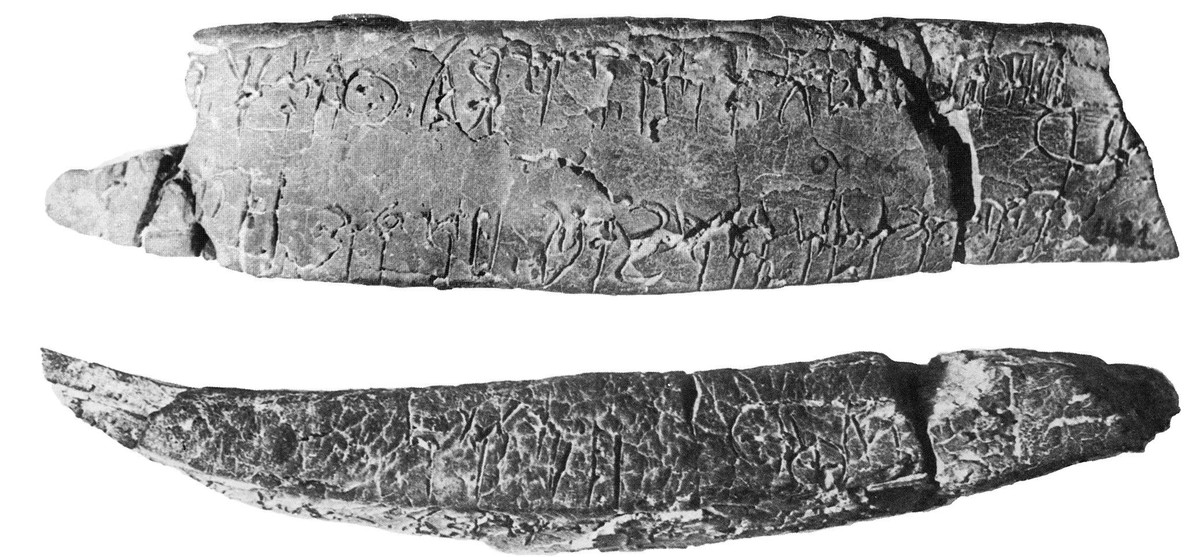
\includegraphics[width=0.7\textwidth]{Images/454.png} % Adjust width and filename
  \caption{Picture of the original document KN Sd 4404.}
  \label{fig:doc6}
\end{figure}

\subsubsection{PY An 657} \label{doc:pyan657}
This document lists various groups of guards and soldiers, together with their numbers, the names of their leaders, and the place of deployment.
Tselentis provides a translation for a small portion of the text containing the name of an "epetas". \\

\textbf{Linear B text}: o-u-ru-to o-pi-ha-ra e-pi-ko-wo ma-re-wo o-ka o-wi-to-no a-pe-ri-ta-wo o-re-ta e-te-wa ko-ki-jo su-we-ro-wi-jo o-wi-ti-ni-jo o-ka-rai VIR 50 ne-da-wa-ta-o o-ka e-ke-me-de a-pi-je-ta ma-ra-te-u ta-ni-ko ha-ru-wo-te ke-ki-de ku-pa-ri-si-jo VIR 20 ai-ta-re-u-si ku-pa-ri-si-jo ke-ki-de VIR 10 \textit{me-ta-qe pe-i e-qe-ta ke-ki-jo} a-e-ri-qo-ta e-ra-po ri-me-ne o-ka-ra o-wi-to-no VIR 30 ke-ki-de-qe a-phu-ka-ne VIR 20 me-ta-qe pe-i ai-ko-ta e-qe-ta \\
\textbf{Greek translation}: \textgreek{Οὖροι Ὀπίχαρα, ἐπίκουροι. Μαλέϝος ὀρχά Ὀϝιτνῶι. Ἀπερίταϝος, Ὀρέλτας, Ἐτέϝας, Κόκκιος, Συϝεροϝιος, Ὀϝιτίνιος. Ὀρχᾶραι: ἄνδρες 50. Νεδαϝάταο ὀρχά. Ἐχεμήδης, Ἀμφιγέτας, Μαλθεύς, Τάνικος. Ἁρυϝότει Κεκκίδες Κυπαρίσσιοι: ἄνδρες 20. Αἰθαλεῦσι Κυπαρίσσιοι Κεκκίδες: ἄνδρες 10. μετά τε σφεῖ ἑπέτας Κέρκιος, Ἀελιπότας, Ἔλαφος. Λιμένει Ὀρχάρα Ὀϝιτνῶι: ἄνδρες 30. Κεκκίδες τε Ἀφυγάνες: ἄνδρες 20. μετά τε σφεῖ Αἰκότας ἑπέτας.} \\
\textbf{English translation}: Guards at Opihara, auxiliaries. Maleus' company at Owitnos. Aperitawos, Orelas, Etewas, Kokkios, Suwerowios, Owitinios. Orcharai: 50 men. Nedawatas' company. Echemedes, Amphigetas, Maltheus, Tanikos. At Harywos, Kekkides Kyparissioi: 20 men. At Aithaleus, Kyparissioi Kekkides: 10 men. And with them, the follower Kerkios, Aelipotas, Elaphos. At Limen, Orchara at Owitnos: 30 men. And Kekkides Aphuganes: 20 men. And with them, Aikotas, the follower.

\paragraph{Analysis.}
Overall, the LLM performs well in recognizing the logical function of the words in the document, despite erroneously treating some of them as proper nouns.
Moreover, it recognizes ethnonyms, but simply transliterates them without attempting to interpret the places to which they relate.

The main terms in this document are:
\begin{itemize}
  \item \textlinb{\Bo\Bu\Bru\Bto} \textlinb{\Be\Bpi\Bko\Bwo} (o-u-ru-to e-pi-ko-wo), "auxiliary guards", from Ancient Greek \textgreek{οὖρος} "guardian" and \textgreek{ἐπίκουρος} "auxiliary".
  \item \textlinb{\Bo\Bpi\Ba2\Bra} (o-pi-ha-ra), is correctly recognized as a place name, but it probably means "at the coast", as also in Homer the term \textgreek{ἐφαλός} is attested, combining the prefix \textgreek{ἐπί} with \textgreek{ἅλς/ἁλός} "sea". 
  \item \textlinb{\Bo\Bka} (o-ka), "company/military unit", corresponds to Ancient Greek \textgreek{ἀρχή}.
  \item \textlinb{\Bo\Bwi\Bto\Bno} (o-wi-to-no), "Owitnos", is correctly identified as a toponym.
  \item \textlinb{\Bo\Bwi\Bto\Bni\Bjo} \textlinb{\Bo\Bwi\Bka\Braiii} (o-wi-ti-ni-jo o-ka-rai), are treated separately by the LLM, but in my opinion they are connected.
  Instead of a proper name, o-wi-ti-ni-jo is probably an ethnonym adjective meaning "of Owitnos", referred to o-ka-rai, which the LLM correctly identifies as a group of people, but not as an ethnic name ("Oihalai", from Tselentis lexicon).
  So they are both ethnonyms.
  \item \textlinb{\Bme\Bta\Bqe} \textlinb{\Bpe\Bi} (me-ta-qe pe-i), "and with them", from Ancient Greek \textgreek{μετά} "with", \textgreek{σφεῖς} "them".
  \item \textlinb{\Be\Bqe\Bta} (e-qe-ta) is a military title meaning "follower/attendant", from Ancient Greek \textgreek{ἑπέτας}.
  \item Other companies, deployed in other locations, are then listed in a similar manner.
  \item \textlinb{\Be\Bra\Bpo} \textlinb{\Bri\Bme\Bne} (e-ra-po ri-me-ne), is completely misinterpreted by the LLM.
  It should be interpreted as "the port of the deers", from Ancient Greek \textgreek{λιμήν} "port" and \textgreek{ἔλαφος} "deers", combined into \textgreek{ἐλάφων λιμένι}.
\end{itemize}

Overall, the high number of proper nouns, ethnonyms and toponyms and the varying structure of the sentences make the translation of this document challenging.

The last part of the document is not straightforward, as it presents two place names (\textit{o-ka-ra} and \textit{o-wi-to-no}) that are close and are assumed to be related, since they also appear together as ethnonyms.
However, I cannot be sure about the correctness of this choice.
Here I report an improved version of the translations, highlighting in red the adjustments and in blue the actual mistakes.
Beware that the last part of the document is uncertain. \\
\textbf{Greek translation}: \textgreek{Οὖροι} \textcolor{blue}{\textgreek{ἐφαλός}}\textgreek{, ἐπίκουροι. Μαλέϝος} \textcolor{red}{\textgreek{ἀρχή}} \textgreek{Ὀϝιτνῷ. Ἀπερίταϝος, Ὀρέλτας, Ἐτέϝας,} \textcolor{red}{\textgreek{Κόλκιος}}\textgreek{, Συϝεροϝιος.} \textcolor{blue}{\textgreek{Ὀϝιτίνιοι Οἰχαλεαι}}\textgreek{: ἄνδρες 50. Νεδαϝάταο} \textcolor{red}{\textgreek{ἀρχή}}\textgreek{. Ἐχεμήδης, Ἀμφιγέτας, Μαλθεύς, Τάνικος.} \textcolor{red}{\textgreek{Ἁρυϝόθεν Κελχίδες Κυπαρίσιοι}}\textgreek{: ἄνδρες 20. Αἰθαλεῦσι} \textcolor{red}{\textgreek{Κελχίδες Κυπαρίσιοι}}\textgreek{: ἄνδρες 10. μετά τε} \textcolor{red}{\textgreek{σφεῖς}} \textgreek{ἑπέτας Κέρκιος. Ἀελιπότας,} \textcolor{blue}{\textgreek{ἐλάφων λιμένι}} \textcolor{red}{\textgreek{Ὀιχαλᾳ}} \textgreek{Ὀϝιτνῷ: ἄνδρες 30.} \textcolor{red}{\textgreek{Κελχίδες}} \textgreek{τε Ἀφυγάνες: ἄνδρες 20. μετά τε} \textcolor{red}{\textgreek{σφεῖς}} \textgreek{Αἰκότας ἑπέτας.} \\
\textbf{English translation}: Guards at \textcolor{blue}{the coast}, auxiliaries. Maleus' company at Owitnos: Aperitawos, Orelas, Etewas, \textcolor{red}{Kolchios}, Suwerowios. \textcolor{blue}{(People) from Owitnos and Oichala}: 50 men. Nedawatas' company. Echemedes, Amphigetas, Maltheus, Tanikos. At Harywos, \textcolor{red}{(people) from Kelchis and Kyparisos}: 20 men. At Aithaleus, \textcolor{red}{(people) from Kelchis and Kyparisos}: 10 men. And with them, the \textcolor{red}{attendant} Kerkios. Aelipotas, \textcolor{blue}{at the deers' port} \textcolor{red}{in Oichala} at Owitnos: 30 men. \textcolor{red}{(People) from Kelchis and Aphy}: 20 men. And with them, Aikotas, the \textcolor{red}{attendant}.

\begin{figure}[H]
  \centering
  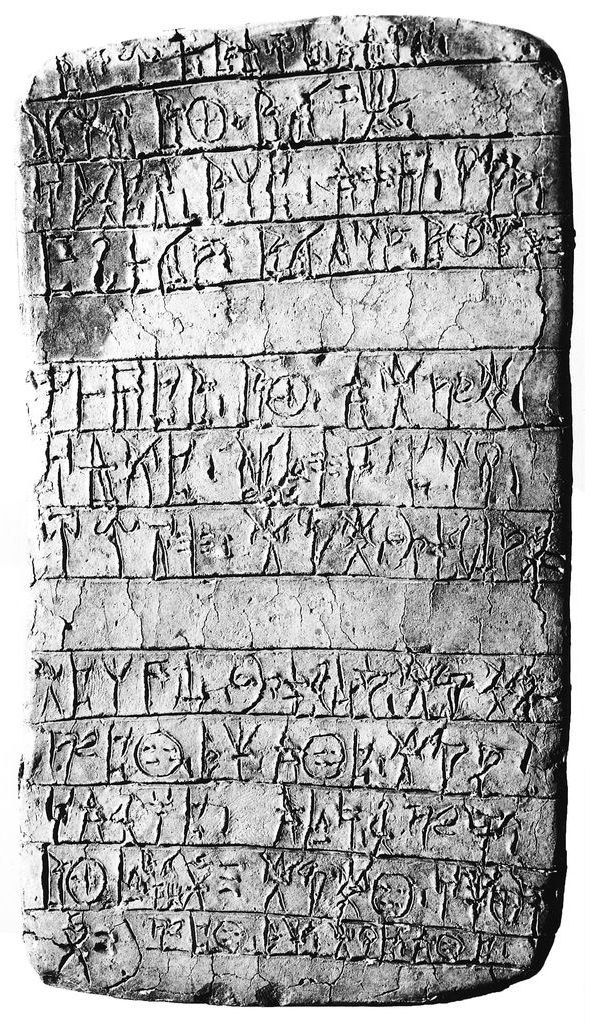
\includegraphics[width=0.4\textwidth]{Images/4726.png} % Adjust width and filename
  \caption{Picture of the original document PY An 657.}
  \label{fig:doc7}
\end{figure}

\subsubsection{PY TA 641} \label{doc:pyta641}
This document is a short inventory of vessels, in particular tripods and pithoi (large storage jars).
The translation provided by Tselentis covers the first portion of the document, while the rest is left untranslated. \\
\textbf{Linear B text}: \textit{ke-re-ha *201VAS [...] ti-ri-po-de ai-ke-u ke-re-si-jo we-ke *201VAS 2 ti-ri-po e-me po-de o-wo-we *201VAS 1 ti-ri-po ke-re-si-jo we-ke a-pu ke-ka-u-me-no} [...] qe-to *203VAS 3 di-pa me-zo-e qe-to-ro-we *202VAS 1 di-pa-e me-zo-e ti-ri-o-we-e *202VAS 2 di-pa me-wi-jo qe-to-ro-we *202VAS 1 di-pa me-wi-jo ti-ri-jo-we *202VAS 1 di-pa me-wi-jo a-no-we *202VAS 1 \\
\textbf{Greek translation}: \textgreek{Σκελέα *201VAS [...] Τρίποδες Αἰγεύς Κρήσιος ἔργε *201VAS 2. Τρίπους ἐν ποδεί ὄϝοϝεις *201VAS 1. Τρίπους Κρήσιος ἔργε ἀπὸ κεκαυμένος. Πίθοι *203VAS 3. Δέπας μεῖζον τετρόϝες *202VAS 1. Δέπαε μείζοε τριόϝεε *202VAS 2. Δέπας μεῖον τετρόϝes *202VAS 1. Δέπας μεῖον τριόϝes *202VAS 1. Δέπας μεῖον ἄνοϝον *202VAS 1.} \\
\textbf{English translation}: Tripod with legs [...] Two tripods, Aigeus, Cretan-made. One tripod, with one foot, one-handled. One tripod, Cretan-made, burnt off. Three jars. One larger, four-handled cup. Two larger, three-handled cups. One smaller, four-handled cup. One smaller, three-handled cup. One smaller, handleless cup.

\paragraph{Analysis.}
In this document, the main problem is the positioning of the first two words, which occur at the beginning of the document but should probably be appended to the end of the first line.
They were added at the top right of the first row, as the scribe likely ran out of space to complete the line.
The translation clearly inherits this misplacement.
A notable aspect of this fragment is the presence of the dual, attested when describing two cups.

The LLM correctly identifies the main words in the document
\begin{itemize}
  \item \textlinb{\Bke\Bre\Bre\Baii} (ke-re-ha), "legs", from Ancient Greek \textgreek{σκελέα}, is a noun, linked to the verb \textit{ke-ka-u-me-no}, specifying where the tripod is burnt.  
  \item \textlinb{\Bti\Bri\Bpo}[\textlinb{\Bde}] (ti-ri-po[-de]), \textlinb{\Bqe\Bto} (qe-to), and \textlinb{\Bdi\Bpa} (di-pa) are the Linear B words for \textgreek{τρίπους} "tripod", \textgreek{πίθος} "jar" and \textgreek{δέπας} "cup", respectively.
  \item \textlinb{\Ba\Bi\Bke\Bu} (ai-ke-u), "Aigeus", is correctly identified as a proper name, despite not being linked to anything precisely, like in Tselentis translation.
  \item \textlinb{\Bke\Bre\Bse\Bi\Bjo} \textlinb{\Bwe\Bke} (ke-re-si-jo we-ke), "Cretan-made", from Ancient Greek \textgreek{Κρήσιος} "Cretan" and \textgreek{ἔργον} "work", is an description linked to the tripods. 
  \item \textlinb{\Be\Bme} \textlinb{\Bpo\Bde} (e-me po-de), "with one foot", from Ancient Greek \textgreek{ἐνί ποδεί}, is another description linked to a tripod.
  It is interesting to note that the LLM correctly interprets \textit{e-me} as the numeral "one", even though it is misinterpreted in the analysis and in the translation.
  \item \textlinb{\Bo\Bwo\Bwe} (o-wo-we), \textlinb{\Bqe\Bto\Bro\Bwe} (qe-to-ro-we), \textlinb{\Bti\Bri\Bjo\Bwe} (ti-ri-o-we-e), and \textlinb{\Ba\Bo\Bno\Be} (a-no-we) are adjectives linked to the jars, meaning "one-handled", "four-handled", "three-handled", and "handleless", respectively.
  \item \textlinb{\Bke\Bka\Bu\Bme\Bno} (ke-ka-u-me-no), "burnt off", from the Ancient Greek verb \textgreek{καίω}, is a perfect passive participle linked to a tripod.
  \item \textlinb{\Bme\Bzo\Be} (me-zo-e) and \textlinb{\Bme\Bwi\Bjo} (me-wi-jo) are adjectives linked to the cups, meaning "larger" and "smaller" from Ancient Greek \textgreek{μείζων} and \textgreek{μείων}, respectively.
\end{itemize}

Here I report a refined version of both translations, adding the first two words at the end of the first line and highlighting in red the adjustments and in blue the mistakes. \\
\textbf{Greek translation}: \textgreek{Τρίποδες Αἰγεύς} \textcolor{red}{\textgreek{Κρήσιου ἔργου}} \textgreek{*201VAS 2. Τρίπους} \textgreek{ἐνί} \textgreek{ποδεί} \textcolor{red}{\textgreek{ὠτόϝεις}} \textgreek{*201VAS 1. Τρίπους} \textcolor{red}{\textgreek{Κρήσιου ἔργου}} \textgreek{κεκαυμένος} \textcolor{blue}{\textgreek{ἀπὸ σκελέα *201VAS}}\textgreek{. Πίθοι *203VAS 3. Δέπας μεῖζον} \textcolor{red}{\textgreek{τετραώτον}} \textgreek{*202VAS 1.} \textcolor{red}{\textgreek{Δέπα μείζονε τριώτω}} \textgreek{*202VAS 2. Δέπας μεῖον} \textcolor{red}{\textgreek{τετραώτον}} \textgreek{*202VAS 1. Δέπας μεῖον} \textcolor{red}{\textgreek{τριώτον}} \textgreek{*202VAS 1. Δέπας μεῖον} \textcolor{red}{\textgreek{ἀνώτον}} \textgreek{*202VAS 1.} \\
\textbf{English translation}: Two tripods, Aigeus, Cretan-made. One tripod, with one foot, one-handled. One tripod, Cretan-made, burnt off \textcolor{blue}{at the legs}. Three jars. One larger, four-handled cup. Two larger, three-handled cups. One smaller, four-handled cup. One smaller, three-handled cup. One smaller, handleless cup.


\begin{figure}[H]
  \centering
  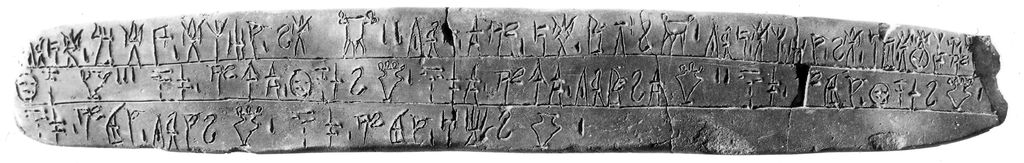
\includegraphics[width=0.7\textwidth]{Images/5344.png} % Adjust width and filename
  \caption{Picture of the original document PY TA 641.}
  \label{fig:doc8}
\end{figure}


\subsubsection{PY Er 312} \label{doc:pyer312}
This document lists various land holdings together with their grain quantities and associated personnel.
Tselentis provides a translation for the entire document.  \\
\textbf{Linear B text}: \textit{wa-na-ka-te-ro te-me-no to-so-jo pe-ma GRA 30 ra-wa-ke-si-jo te-me-no GRA 10 te-re-ta-o to-so pe-ma GRA 30 to-so-de te-re-ta VIR 3 wo-ro-ki-jo-ne-jo e-re-mo to-so-jo pe-ma GRA 6} \\
\textbf{Greek translation}: \textgreek{ϝανακτέρον τέμενος: τοσοῖο σπέρματος ΓΡΑ 30. λαϝαγεσίοιο τέμενος: ΓΡΑ 10. τελεσταῶν τόσον σπέρμα: ΓΡΑ 30. τοσόνδε τελεσταί: ΑΝΗΡ 3. ϝοργιονείοιο ἔρημον: τοσοῖο σπέρματος ΓΡΑ 6.} \\
\textbf{English translation}: Royal temenos: of so much grain, GRA 30. Temenos of the lawagetas: GRA 10. Of the telestai, so much grain: GRA 30. And so many telestai: 3 men. Fallow land of Worgion: of so much grain, GRA 6.

\paragraph{Analysis.} The LLM performs well in recognizing all the words in the document.
It also recognizes the logograms in its analysis, although it simply transliterates them in the translation.
The translation is accurate overall, helped by the clear, list-like structure of the entries.
The main terms are:
\begin{itemize}
  \item \textlinb{\Bte\Bme\Bno} (te-me-no), "temenos", from Ancient Greek \textgreek{τέμενος}. Its usual meaning is "sacred precinct", but here it is used for a land holding.
  The two occurrences are modified by \textlinb{\Bwa\Bna\Bka\Bte\Bro} (wa-na-ka-te-ro), "royal", transliterated as \textgreek{ϝανακτέρος} from \textgreek{ἄναξ}, and \textlinb{\Bra\Bwa\Be\Bke\Bsi\Bjo} (ra-wa-ke-si-jo), "of the lawagetas", a Mycenaean official title, transliterated as \textgreek{λαϝαγεσίοιο}.
  \item \textlinb{\Bto\Bo\Bso\Bo\Bjo} (to-so-jo), "of so much", from Ancient Greek \textgreek{τόσοιο}, functions as a genitive of measure linked to the quantity of grain.
  It is therefore associated with \textlinb{\Bpe\Bma} (pe-ma), "grain/seed", from \textgreek{σπέρμα}, and with the logogram \textit{GRAnum} for "grain".
  \item \textlinb{\Bte\Bre\Bta}[\textlinb{\Bo}] (te-re-ta[-o]), "telestai", from \textgreek{τελεσταί}, a Mycenaean title possibly connected with \textgreek{τέλος} "tax". In later Greek the term can denote a "priest".
  \item \textlinb{\Bwo\Bro\Bki\Bo\Bjo\Bne\Bjo} \textlinb{\Be\Bre\Bmo} (wo-ro-ki-jo-ne-jo e-re-mo) is the only imprecise part of the translation.
  Tselentis associates this expression with a cult site; thus the translation should be "remote place of the Worgiones", from \textgreek{ἔρημος} "remote place."

\end{itemize}
Here I provide a slightly refined version of both translations, highlighting in red the few adjustments. \\
\textbf{Greek translation}: \textgreek{ϝανακτέρον τέμενος: τοσοῖο σπέρματος} \textcolor{red}{\textgreek{ΣΙΤΟΣ}} \textgreek{30. λαϝαγεσίοιο τέμενος:} \textcolor{red}{\textgreek{ΣΙΤΟΣ}} \textgreek{10. τελεσταῶν τόσον σπέρμα:} \textcolor{red}{\textgreek{ΣΙΤΟΣ}} \textgreek{30. τοσόνδε τελεσταί: ΑΝΗΡ 3.} \textcolor{blue}{\textgreek{ϝοργιώνειοιον}} \textgreek{ἔρημον: τοσοῖο σπέρματος} \textcolor{red}{\textgreek{ΣΙΤΟΣ}} \textgreek{6.} \\
\textbf{English translation}: Royal \textcolor{red}{land holding}: of so much grain, 30 \textcolor{red}{units of grain}. \textcolor{red}{Land holding} of the lawagetas: 10 \textcolor{red}{units of grain}. Of the telestai, so much grain: 30 \textcolor{red}{units of grain}. And so many telestai: 3 men. \textcolor{blue}{Remote land of the Worgiones}: of so much grain, 6 \textcolor{red}{units of grain}.

\begin{figure}[H]
  \centering
  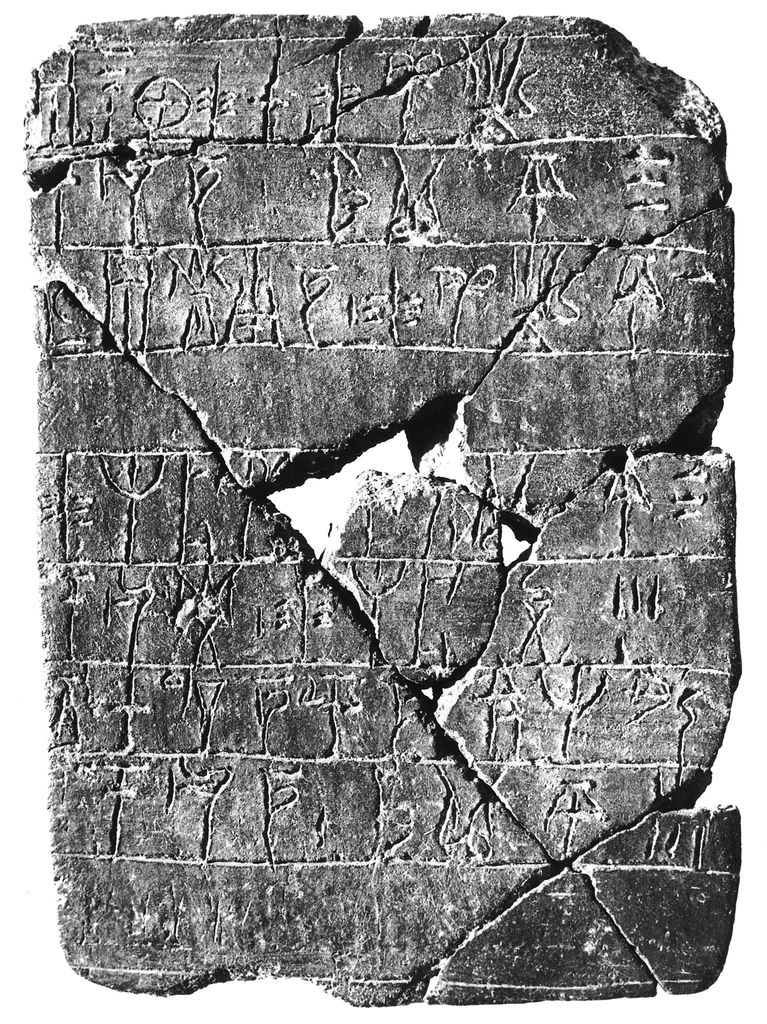
\includegraphics[width=0.38\textwidth]{Images/4959.png} % Adjust width and filename
  \caption{Picture of the original document PY Er 312.}
  \label{fig:doc9}
\end{figure}

\subsubsection{KN Fp 1+31}
This document records oil offerings made in the month of Deukios.
In this case, Tselentis provides a translation covering the whole document. \\
\textbf{Linear B text}: \textit{de-u-ki-jo-jo me-no di-ka-ta-jo di-we OLE S 1 da-da-re-jo-de OLE S 2 pa-de OLE S 1 pa-si-te-o-i OLE 1 qe-ra-si-ja OLE S 1 [...] a-mi-ni-so pa-si-te-o-i S 1 [...] e-ri-nu OLE V 3 *47-da-de OLE V 1 a-ne-mo i-je-re-ja V 4 to-so OLE 3 S 2 V 2} \\
\textbf{Greek translation}: \textgreek{Δευκίοιο μηνός: Δικταίῳ Διϝεῖ ΕΛΑΙΟΝ S 1. Δαδαλείονδε ΕΛΑΙΟΝ S 2. Πάνδει ΕΛΑΙΟΝ S 1. πασιθεοῖς ΕΛΑΙΟΝ 1. Θηρασίᾳ ΕΛΑΙΟΝ S 1 [...] Ἀμνισός: πασιθεοῖς S 1 [...] Ἐρινύι ΕΛΑΙΟΝ V 3. Οὐδαδε ΕΛΑΙΟΝ V 1. ἀνέμοιο ἱερείᾳ V 4. τόσον ΕΛΑΙΟΝ 3 S 2 V 2.} \\
\textbf{English translation}: In the month of Deukios: To Dictaean Zeus: 1 S unit of oil. To the Daedaleion: 2 S units of oil. To Pandes: 1 S unit of oil. To all gods: 1 unit of oil. To Therasia: 1 S unit of oil. [...] Amnisos: To all gods: 1 S unit (of oil). [...] To Erinys: 3 V units of oil. To Oudade: 1 V unit of oil. To the priestess of the wind: 4 V units (of oil). Total oil: 3 units, 2 S units, 2 V units.

\paragraph{Analysis.}
The translation of this document is quite accurate: the main terms and phrases are correctly rendered, and the overall structure is preserved.
This success largely reflects the document's highly regular format, which repeats the same pattern several times.

The main words that appear in this document are:
\begin{itemize}
\item \textlinb{\Bde\Bu\Bki\Bjo\Bjo} (de-u-ki-jo-jo) "of Deukios", linked to Ancient Greek \textgreek{Δευκίος}, the name of a month in the Mycenaean calendar.
This reading is confirmed by the following word \textlinb{\Bme\Bno} (me-no) "month", from Ancient Greek \textgreek{μήν}.
\item The recipients of the offerings are all in the dative case.
The first is \textlinb{\Bdi\Bka\Bta\Bjo} \textlinb{\Bdi\Bwe} (di-ka-ta-jo di-we), corresponding to Ancient Greek \textgreek{Ζεύς/Διός} with the epithet \textgreek{Δικταίος}.
The LLM associates this with Mount Dicte in Crete; Tselentis, however, writes simply "Dikatios".
\item \textlinb{\Bda\Bda\Bre\Bjo\Bde} (da-da-re-jo-de) is correctly recognized as a place-name.
The LLM renders it as the more generic "Daedaleion", while Tselentis gives "the city of Daidalos".
\item \textlinb{\BUvi\Bda\Bde} (*47-da-de) is transliterated by the LLM as "Oudade", but the initial syllabogram has no agreed phonetic value in the literature.
\item \textlinb{\Ba\Bne\Bmo} (a-ne-mo) "of the wind", from Ancient Greek \textgreek{ἄνεμος}, is correctly identified as a genitive; however, it is probably better analyzed as plural rather than singular.
\end{itemize}

In light of the above considerations, I report an improved version of both translations, highlighting in red the adjustments. \\
\textbf{Greek translation}: \textgreek{Δευκίοιο μηνός: Δικταίῳ Διϝεῖ ΕΛΑΙΟΝ S 1. Δαδαλείονδε ΕΛΑΙΟΝ S 2. Πάνδει ΕΛΑΙΟΝ S 1.} \textcolor{red}{\textgreek{πάσι θεοῖς}} \textgreek{ΕΛΑΙΟΝ 1. Θηρασίᾳ ΕΛΑΙΟΝ S 1 [...] Ἀμνισός:} \textcolor{red}{\textgreek{πάσι θεοῖς}} \textgreek{[...] Ἐρινύι ΕΛΑΙΟΝ V 3.} \textcolor{red}{\textgreek{*47-δαδε}} \textgreek{ΕΛΑΙΟΝ V 1.} \textcolor{red}{\textgreek{ἀνέμων}} \textgreek{ἱερείᾳ V 4. τόσον ΕΛΑΙΟΝ 3 S 2 V 2.} \\
\textbf{English translation}: In the month of Deukios: To Dictaean Zeus: 1 S unit of oil. To the \textcolor{red}{city of Daidalos}: 2 S units of oil. To Pandes: 1 S unit of oil. To all gods: 1 unit of oil. To Therasia: 1 S unit of oil. [...] Amnisos: To all gods: 1 S unit (of oil). [...] To Erinys: 3 V units of oil. To \textcolor{red}{?-dade}: 1 V unit of oil. To the priestess of the \textcolor{red}{winds}: 4 V units (of oil). Total oil: 3 units, 2 S units, 2 V units.

\begin{figure}[H]
  \centering
  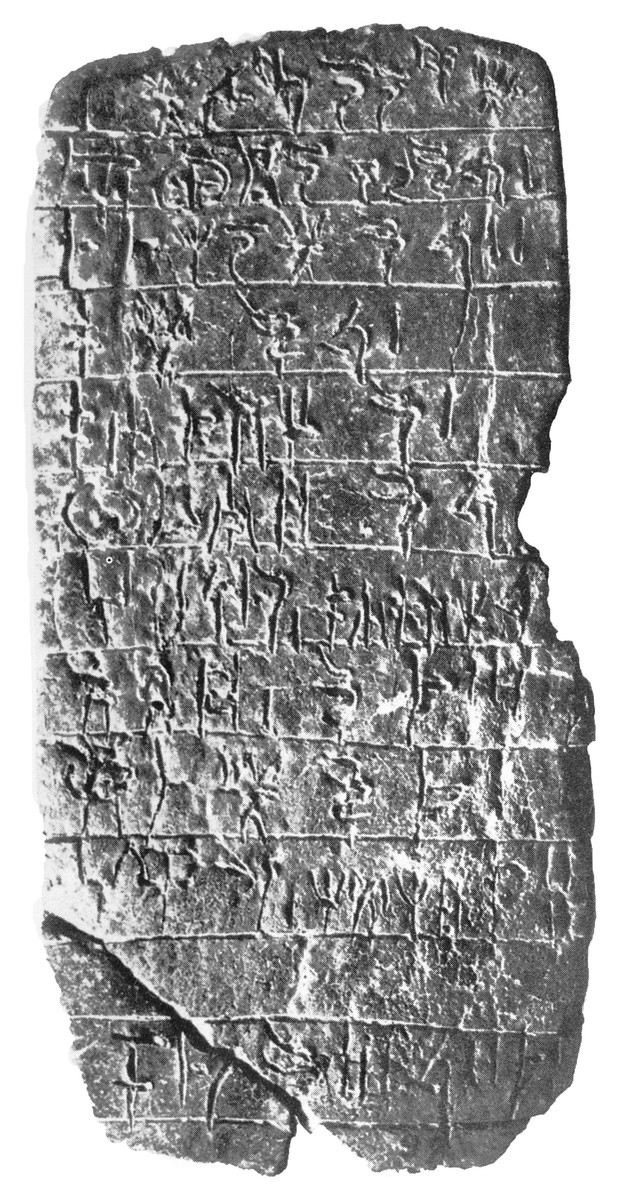
\includegraphics[width=0.38\textwidth]{Images/4088.png} % Adjust width and filename
  \caption{Picture of the original document KN Fp 1+31.}
  \label{fig:doc10}
\end{figure}

\subsubsection{PY Ab 573}
This very short document lists women and children, as well as quantities of grain and figs.
Tselentis provides a translation for a small portion of the document. \\
\textbf{Linear B text}: GRA 5 T 1 DA TA \textit{pu-ro mi-ra-ti-ja MUL 16 ko-wa 3 ko-wo 7} NI 5 1 \\
\textbf{Greek translation}: \textgreek{Πύλος: ΣΙΤΟΣ 5 T 1 DA TA. Μιλατίαι ΓΥΝΗ 16, κόρϝαι 3, κόρϝοι 7. ΣΥΚΟΝ 5 1.} \\
\textbf{English translation}: Pylos: Grain 5 T 1. DA TA. Milatian women: 16 women, 3 girls, 7 boys. Figs: 5 1.

The initial part of the document is not translated by Tselentis. It is written at the top of the tablet, as if the scribe had run out of space to complete the line.
It should probably be appended at the end of the line.
However, it is likely independent of the rest of the entry, so the LLM's placement is acceptable.

\paragraph{Analysis.}
This document is rich in logograms: the only syllabographic words are the ethnonym \textlinb{\Bmi\Bra\Bti\Bja} (mi-ra-ti-ja) from Ancient Greek \textgreek{Μιλήσιαι} "miletian", and \textlinb{\Bko\Bwo}/\textlinb{\Bko\Bwa} (ko-wo/ko-wa) from Ancient Greek \textgreek{κόρος/κόρη} "boy/girl".
The LLM correctly identifies the remaining items as logograms or abbreviations.
The translation is accurate, with a minor adjustment shown below in red. \\
\textbf{Greek translation}: \textgreek{Πύλος: ΣΙΤΟΣ 5 T 1 DA TA.} \textcolor{red}{\textgreek{Μιλήσιαι}} \textgreek{ΓΥΝΗ 16, κόρϝαι 3, κόρϝοι 7. ΣΥΚΟΝ 5 1.} \\
\textbf{English translation}: Pylos: Grain 5 T 1. DA TA. \textcolor{red}{Miletian} women: 16 women, 3 girls, 7 boys. Figs: 5 1.

\begin{figure}[H]
  \centering
  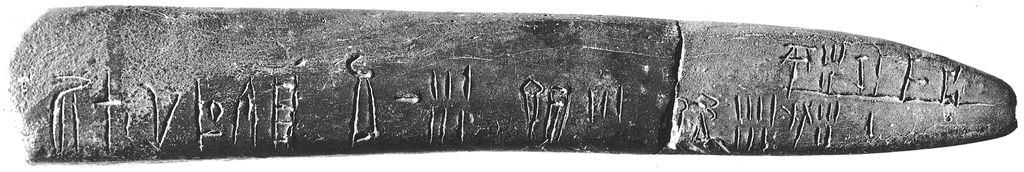
\includegraphics[width=0.7\textwidth]{Images/4611.png} % Adjust width and filename
  \caption{Picture of the original document PY Ab 573.}
  \label{fig:doc11}
\end{figure}

\subsubsection{PY Un 718} \label{doc:pyun718}
This final document is an administrative record listing offerings.
The translation provided by Tselentis for this document covers only the first part of the tablet. \\
\textbf{Linear B text}: \textit{sa-ra-pe-da po-se-da-o-ni do-so-mo o-wi-de-ta-i do-so-mo to-so e-ke-rya-wo do-se GRA 4 VIN 3 BOSm 1} tu-ryo TU+RYO 10 ko-wo *153 1 me-ri-to V 3 o-da-ha da-mo GRA 2 VIN 2 OVISm 2 TU+RYO 5 a-re-ro A+RE+PA V 2 *153 1 to-so-de ra-wa-ke-ta do-se OVISm 2 me-re-u-ro FAR T 6 VIN S 2 o-da-ha wo-ro-ki-jo-ne-jo ka-ma GRA [...] T 6 VIN S 1 TU+RYO 5 me-ri [...] 1 [...] V 1 \\
\textbf{Greek translation}: \textgreek{Σραπέδας: δόσμος Ποσειδῶνι. δόσμος οϝιδετται. Τόσος Ἐχελαϝῶν δώσει: ΣΙΤΟΣ 4, ΟΙΝΟΣ 3, ΤΑΥΡΟΣ 1, τυρίον ΤΥΡΙΟΝ 10, κοῦρος *153 1, μέλι V 3. Οδαhα δᾶμος: ΣΙΤΟΣ 2, ΟΙΝΟΣ 2, ΚΡΙΟΣ 2, ΤΥΡΙΟΝ 5. Ἀλεῖρος: ἀλειφάρ V 2, *153 1. Τοσόνδε λαϝαγέτας δώσει: ΚΡΙΟΣ 2, ἄλευρον ΦΑΡ T 6, ΟΙΝΟΣ S 2. Οδαhα ϝρογιονείον κᾶμα: ΣΙΤΟΣ [...] T 6, ΟΙΝΟΣ S 1, ΤΥΡΙΟΝ 5, μέλι [...] 1 [...] V 1.}
\textbf{English translation}: Sarapeda: Offering to Poseidon. Offering to the overseers. Echelawa will give this much: Grain 4, Wine 3, Bull 1, Cheese 10, Boy *153 1, Honey V 3. Also, the community: Grain 2, Wine 2, Ram 2, Cheese 5. Aleiros: Ointment V 2, *153 1. This much the Lawagetas will give: Ram 2, Flour T 6, Wine S 2. Also, Wrogioneios' plot: Grain [...] T 6, Wine S 1, Cheese 5, Honey [...] 1 [...] V 1.

\paragraph{Analysis.}
The LLM provides a fairly accurate translation of this document, with some problematic issues.
\begin{itemize}
  \item The first word \textlinb{\Bsa\Bra\Be\Bpe\Bda} (sa-ra-pe-da) is transliterated as "Sarapeda". The LLM considers it as a proper noun or a toponym. Its possible toponym function is mentioned also by Chadwick and Ventris in their lexicon \cite{chadwick-notes}.
  The LLM treats it as a proper noun or toponym, a possibility also noted by Chadwick and Ventris \cite{chadwick-notes}. Tselentis, however, interprets it as an epithet of Poseidon (the following word \textlinb{\Bpo\Bse\Bda\Bo\Bni} po-se-da-o-ni, \textgreek{Ποσειδῶν}) and translates "Srapedas".
  \item The word \textlinb{\Bo\Bwi\Bde\Bta\Bi} (o-wi-de-ta-i) is clearly linked to Ancient Greek \textgreek{οἶδα} "to know".
  Tselentis treats it as a religious title and leaves it transliterated; the LLM renders it as "overseers". In any case, the dative plural is correctly recognized.
  \item The verb \textlinb{\Bdo\Bse} (do-se) is correctly identified as the 3rd person singular future active indicative of the Ancient Greek verb \textgreek{δίδωμι}, "to give".
  \item A notable feature of the enumerated items in this fragment is the logographic merging of common Linear B words, which the LLM successfully reconstructs.
  For example, the word \textlinb{\Btu\Broii} (tu-ryo) appears both as a word and as the fused sign (TU+RYO) for "cheese", from Ancient Greek \textgreek{τυρίον}. 
  Conversely, \textlinb{\Ba\Bre\Bpa} (a-re-pa) appears only as the logogram (A+RE+PA) for "ointment", from Ancient Greek \textgreek{ἀλείφαρ}.
  \item The meaning of \textlinb{\Bko\Bwo}, paired with the unknown syllabogram *153, is uncertain.
  \item \textlinb{\Bo\Bda\Baii} (o-da-ha) is treated as a conjunction "also", which matches Tselentis' description as an introductory word.
  \item \textlinb{\Bwo\Bro\Bki\Bjo\Bne\Bjo} \textlinb{\Bka\Bma} (wo-ro-ki-jo-ne-jo ka-ma) refers again to the Worgiones cult association, as in Document \hyperref[doc:pyer312]{PY Er 312}.
  \textit{ka-ma} is correctly taken as "plot/field", from Ancient Greek \textgreek{κτῆμα}.
\end{itemize}

Here I report a refined version of both translations, highlighting in red the adjustments. \\
\textbf{Greek translation}: \textgreek{Δόσμος} \textcolor{red}{\textgreek{Σραπέδᾳ}} \textgreek{Ποσειδῶνι. Δόσμος} \textcolor{red}{\textgreek{οϝιδέταις}}\textgreek{. Τόσος Ἐχελαϝῶν δώσει: ΣΙΤΟΣ 4, ΟΙΝΟΣ 3, ΤΑΥΡΟΣ 1, τυρίον ΤΥΡΙΟΝ 10, κοῦρος *153 1, μέλι V 3. Οδαhα δᾶμος: ΣΙΤΟΣ 2, ΟΙΝΟΣ 2, ΚΡΙΟΣ 2, ΤΥΡΙΟΝ 5. Ἀλεῖρος: ἀλειφάρ V 2, *153 1. Τοσόνδε λαϝαγέτας δώσει: ΚΡΙΟΣ 2, ἄλευρον} \textcolor{red}{\textgreek{ΑΛΕΥΡΟΝ}} \textgreek{T 6, ΟΙΝΟΣ S 2. Οδαhα} \textcolor{red}{\textgreek{ϝοργιονείον κτῆμα}}\textgreek{: ΣΙΤΟΣ [...] T 6, ΟΙΝΟΣ S 1, ΤΥΡΙΟΝ 5, μέλι [...] 1 [...] V 1.} \\
\textbf{English translation}: Offering to \textcolor{red}{Srapedas} Poseidon. Offering to the overseers. \textcolor{red}{Echelawon} will give this much: Grain 4, Wine 3, Bull 1, Cheese 10, Boy *153 1, Honey V 3. Also, the community: Grain 2, Wine 2, Ram 2, Cheese 5. Aleiros: Ointment V 2, *153 1. This much the Lawagetas will give: Ram 2, Flour T 6, Wine S 2. Also, the plot \textcolor{red}{of the Worgiones}: Grain [...] T 6, Wine S 1, Cheese 5, Honey [...] 1 [...] V 1.

\begin{figure}[H]
  \centering
  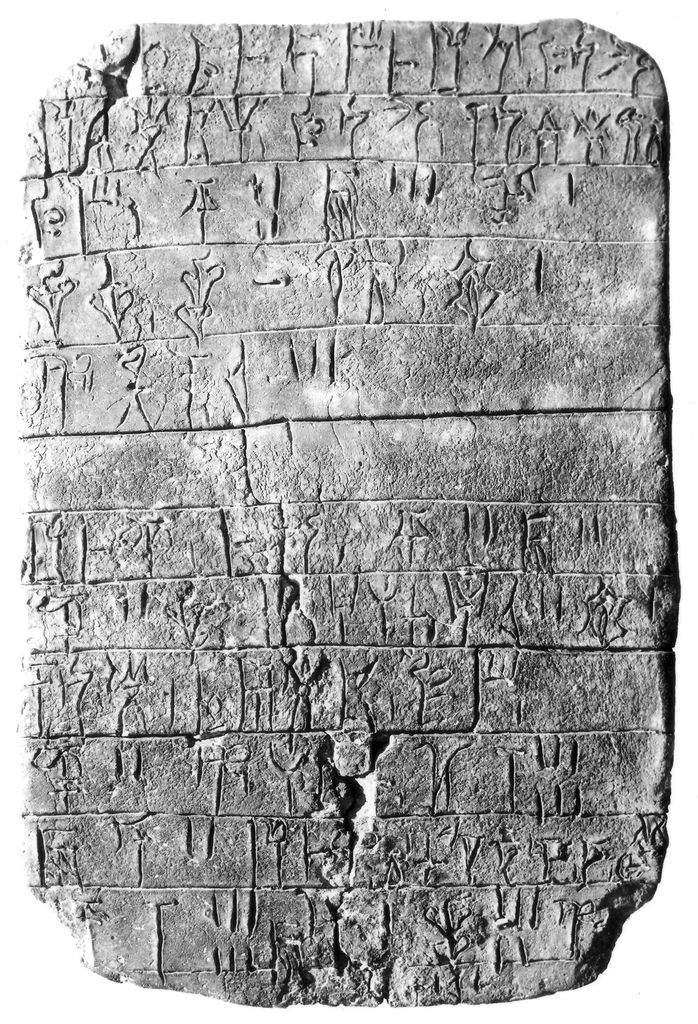
\includegraphics[width=0.45\textwidth]{Images/5385.png} % Adjust width and filename
  \caption{Picture of the original document PY Un 718.}
  \label{fig:doc12}
\end{figure}

The translations of all remaining documents are provided in the thesis files, in a CSV file that includes the document index, the Linear B form, the Greek and English translations, and the model's reasoning.

\subsection{Error Analysis} \label{sec:errors}
This section summarizes the errors made by the LLM in translating the selected documents and analyzes their likely causes, given the input information.

The first type of error arises from misinterpreting words when cognate support is insufficient or misleading.
This is especially likely when no clear Ancient Greek cognate exists or when the cognate's meaning has shifted.
For example, in Document \hyperref[doc:pyjn310]{Py Jn 310} the form \textlinb{\Bpo\Bti\Bni\Bja\Bwe\Bjo} (po-ti-ni-ja-we-jo) is not treated as place-related, because Ancient Greek \textgreek{πότνια} ("mistress/lady") no longer transparently denotes a deity.
Another example appears in Document \hyperref[doc:knso4439]{KN So 4439}, where \textlinb{\Be\Bri\Bka} (e-ri-ka) is associated with Ancient Greek \textgreek{ἑλικτός} "twisted", unlike in Linear B, where it is associated with the willow tree.

A second type of error is the misinterpretation of a word's grammatical function.
This can occur when the LLM fails to recognize a noun's case or a verb's tense.
For instance, in document \hyperref[doc:pyan657]{PY An 657}, \textlinb{\Be\Bra\Bwo} (e-ra-wo) is treated as a nominative noun, whereas it is actually genitive.
Another example is in document \hyperref[doc:pyta641]{PY TA 641}, where \textlinb{\Bke\Bre\Baii} (ke-re-ha), from Ancient Greek \textgreek{σκέλεα} "legs", is not associated with its particle \textgreek{ἀπό}; however, this error is likely attributable to the unusual placement of the initial line in the document.

The third error type I want to highlight is the misinterpretation of a word's function due to misclassification.
When the auxiliary classifiers mislabel a word, the LLM may misassign its role in the sentence.
For example, in Document \hyperref[doc:pyan657]{PY An 657}, two ordinary locatives are interpreted as proper toponyms: both \textlinb{\Bo\Bpi\Baii\Bra} (o-pi-ha-ra) and \textlinb{\Bri\Bme\Bne} (ri-me-ne) are rendered as "Opihara" and "Limenei", rather than "at the coast" and "at the port".
Likewise, the two occurrences of \textlinb{\Bwo\Bro\Bki\Bjo\Bne\Bjo} (wo-ro-ki-jo-ne-jo) in Documents \hyperref[doc:pyer312]{PY Er 312} and \hyperref[doc:pyun718]{PY Un 718} are misclassified as a proper name, which leads to an interpretation as an anthroponym rather than as a cult association.

Finally, some errors arise from the LLM's difficulty in interpreting certain logographic abbreviations, which are occasionally misread or left unspecified.
Taken together, these are the main error patterns observed in the analyzed documents, given the input information available to the model.

A further, notable issue is the LLM's tendency to produce forms closer to Mycenaean than to classical Ancient Greek.
Many translations retain clear Linear B reminiscences, most notably the persistent use of the digamma (\textgreek{ϝ}) and frequent Mycenaean case endings.
I have largely set these aside when the sense was clear and the content was correctly interpreted.
However, if classical Ancient Greek is to serve as a reliable support language for translation, the system will need better normalization toward Classical morphology and orthography (e.g., consistent suppression of \textgreek{ϝ} where appropriate and alignment with Classical inflectional endings).

\subsection{Machine translation metrics} \label{sec:metrics}
To quantitatively evaluate the LLM's translation performance, I computed several machine translation metrics comparing the LLM's output with my revised translations.
The metrics used are:
\begin{itemize}
  \item \textbf{BLEU (Bilingual Evaluation Understudy)} \cite{bleu}: Measures modified n\mbox{-}gram precision between the system output and a reference, with a brevity penalty to discourage overly short translations. Scores typically range from 0 to 1; higher is better.
  \item \textbf{METEOR (Metric for Evaluation of Translation with Explicit ORdering)} \cite{meteor}: Uses a precision-recall harmonic mean (with recall weighting), aligns words via stemming/synonyms, and applies a fragmentation penalty for disordered matches. Ranges from 0 to 1; higher is better.
  \item \textbf{ROUGE (Recall-Oriented Understudy for Gisting Evaluation)} \cite{rouge}: A recall-oriented family measuring overlap with the reference. ROUGE-1 and ROUGE-2 target unigram and bigram overlap; ROUGE-L uses the longest common subsequence. Scores range from 0 to 1; higher is better.
  \item \textbf{TER (Translation Edit Rate)} \cite{ter}: The number of edits (insertions, deletions, substitutions, and shifts) needed to transform the system output into the reference, normalized by reference length. $0$ is perfect; lower is better (and values can exceed 1 on very poor outputs).
  \item \textbf{CHRF (Character F-score)} \cite{chrf}: Computes an F-score over character n-grams, capturing fine-grained matches and being robust to inflectional variation. Ranges from 0 to 1; higher is better.
  \item \textbf{WER (Word Error Rate)} \cite{wer}: Word-level edit rate $(S{+}D{+}I)/N$ (substitutions, deletions, insertions over reference length). $0$ is perfect; lower is better (and values can exceed 1 on very poor outputs).
\end{itemize}

\subsubsection{Results}
Table \ref{tab:metrics-combined} reports the averaged evaluation scores across all 12 documents, 
for both Ancient Greek and English translations. 

\begin{table}[H]
\centering
\caption{Evaluation metrics for Ancient Greek and English translations (averaged over 12 documents).}
\label{tab:metrics-combined}
\begin{tabular}{|l|c|c|}
\hline
Metric & Greek & English \\
\hline
BLEU        & 0.641 & 0.768 \\
METEOR      & 0.813 & 0.880 \\
ROUGE-1 F1  & 0.818 & 0.903 \\
ROUGE-2 F1  & 0.698 & 0.837 \\
ROUGE-L F1  & 0.815 & 0.899 \\
TER         & 0.187 & 0.158 \\
CHRF        & 0.836 & 0.848 \\
WER         & 0.189 & 0.161 \\
\hline
\end{tabular}
\end{table}

Overall, the LLM's translations are quite accurate, with English outperforming Greek across all metrics.
The BLEU scores of 0.641 for Greek and 0.768 for English, however, derive from the LLM's tendency to retain Mycenaean features, which I have not even fully corrected in my revised translations.
However, these reconstructions are still quite close to the Ancient Greek forms, as reflected in the high CHRF scores (0.836 for Greek and 0.848 for English), which capture character-level matches and are more robust to inflectional variations.